%
% Copyright 2018 Joel Feldman, Andrew Rechnitzer and Elyse Yeager.
% This work is licensed under a Creative Commons Attribution-NonCommercial-ShareAlike 4.0 International License.
% https://creativecommons.org/licenses/by-nc-sa/4.0/
%
\questionheader{ex:s1.11}

\noindent
Recall that we are using $\log x$ to denote the logarithm of $x$ with
base $e$. In other courses it is often denoted $\ln x$.


%%%%%%%%%%%%%%%%%%
\subsection*{\Conceptual}
%%%%%%%%%%%%%%%%%%
\begin{Mquestion}
Suppose we approximate an object to have volume $1.5 \mathrm{m}^3$, when its exact volume is $1.387 \mathrm{m}^3$. Give the relative error, absolute error, and percent error of our approximation.
\end{Mquestion}
\begin{hint}
The absolute error is  the difference of the two values; the relative error is the absolute error divided by the exact value; the percent error is one hundred times the relative error.
\end{hint}
\begin{answer}
Relative error: $\approx 0.08147$; absolute error: $0.113$; percent error: $\approx 8.147\%$.
\end{answer}
\begin{solution}
The absolute error is the difference between the two values:
\[|1.387-1.5| = 0.113\]
The relative error is the absolute error divided by the exact value:
\[\frac{0.113}{1.387}\approx 0.08147\]
The percent error is 100 times the relative error:
\[\approx 8.147\%\]
\end{solution}
%%%%%%%%%%%%%%%%%%%
\begin{question}
Consider approximating $\displaystyle\int_2^{10} f(x)~\dee{x}$, where $f(x)$ is the function in the graph below.
\begin{center}
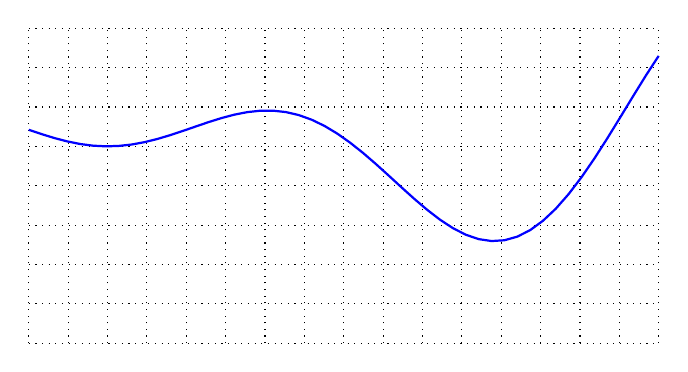
\begin{tikzpicture}
\YEaaxis{1.25}{7.25}{1.25}{3.25}
\draw[dotted] (-1,-1) grid[step=0.5] (7,3);
\YExcoord{1}{2}
\YExcoord{5}{10}
\draw[thick, blue] plot[domain=-1:7, samples=50](\x,{.25*\x* sin(\x r)+1.5});
\end{tikzpicture}
\end{center}
\begin{enumerate}[(a)]
\item Draw the rectangles associated with the midpoint rule approximation and $n=4$.
\item Draw the trapezoids associated with the trapezoidal rule approximation and $n=4$.
\end{enumerate}
You don't have to give an approximation.
\end{question}
\begin{hint}
You should have four rectangles in one drawing, and four trapezoids in another.
\end{hint}
\begin{answer}
Midpoint rule:
\begin{center}
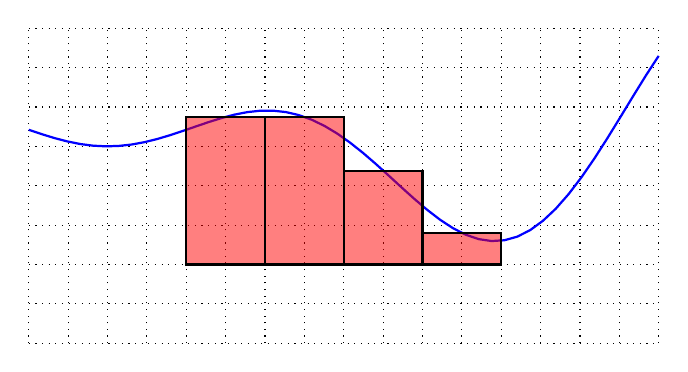
\begin{tikzpicture}
\YEaaxis{1.25}{7.25}{1.25}{3.25}
\draw[dotted] (-1,-1) grid[step=0.5] (7,3);
\YExcoord{1}{2}
\YExcoord{5}{10}
\draw[thick, blue] plot[domain=-1:7, samples=50](\x,{.25*\x* sin(\x r)+1.5});
\draw[thick, black, fill=red, fill opacity=0.5] (1,0) rectangle (2,1.87)
(2,0) rectangle (3,1.87)
(3,0) rectangle (4,1.19)
(4,0) rectangle (5,0.4);
\end{tikzpicture}
\end{center}
Trapezoidal rule:
\begin{center}
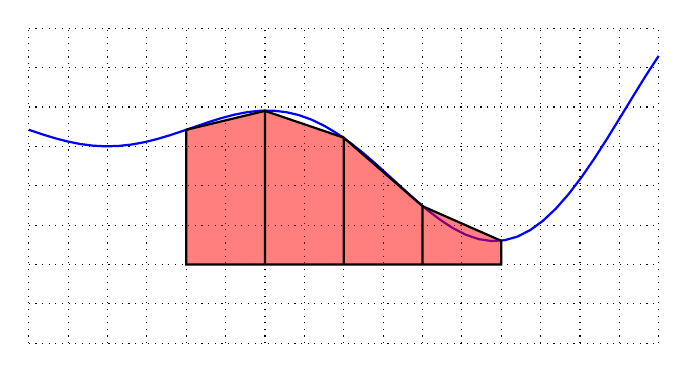
\begin{tikzpicture}
\YEaaxis{1.25}{7.25}{1.25}{3.25}
\draw[dotted] (-1,-1) grid[step=0.5] (7,3);
\YExcoord{1}{2}
\YExcoord{5}{10}
\draw[thick, blue] plot[domain=-1:7, samples=50](\x,{.25*\x* sin(\x r)+1.5});
\filldraw[thick, black, fill=red, fill opacity=0.5]
(1,0)--(1,1.71)--(2,1.95)|-cycle
(2,0)--(2,1.95)--(3,1.61)|-cycle
(3,0)--(3,1.61)--(4,0.74)|-cycle
(4,0)--(4,0.74)--(5,0.3)|-cycle;
\end{tikzpicture}
\end{center}
\end{answer}
\begin{solution}
Midpoint rule:
\begin{center}
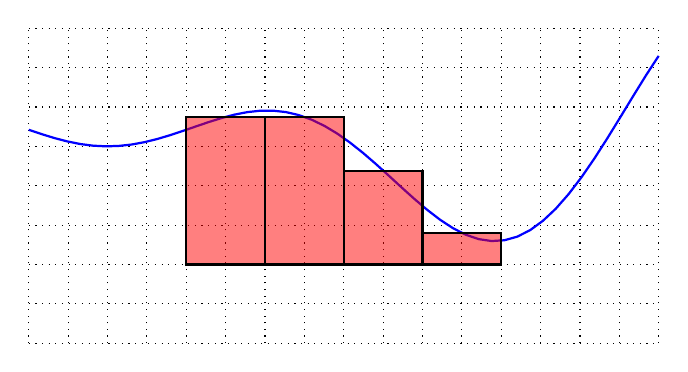
\begin{tikzpicture}
\YEaaxis{1.25}{7.25}{1.25}{3.25}
\draw[dotted] (-1,-1) grid[step=0.5] (7,3);
\YExcoord{1}{2}
\YExcoord{5}{10}
\draw[thick, blue] plot[domain=-1:7, samples=50](\x,{.25*\x* sin(\x r)+1.5});
\draw[thick, black, fill=red, fill opacity=0.5] (1,0) rectangle (2,1.87)
(2,0) rectangle (3,1.87)
(3,0) rectangle (4,1.19)
(4,0) rectangle (5,0.4);
\end{tikzpicture}
\end{center}
Trapezoidal rule:
\begin{center}
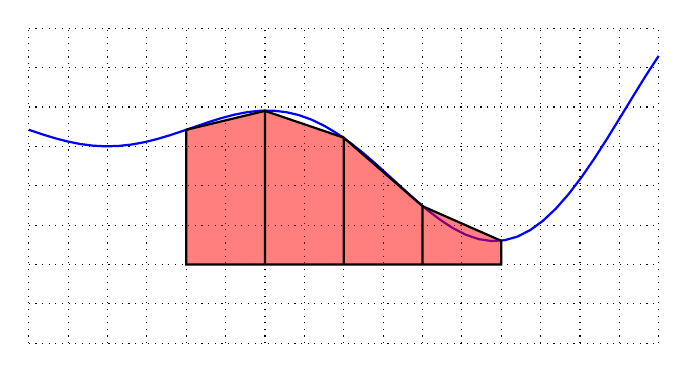
\begin{tikzpicture}
\YEaaxis{1.25}{7.25}{1.25}{3.25}
\draw[dotted] (-1,-1) grid[step=0.5] (7,3);
\YExcoord{1}{2}
\YExcoord{5}{10}
\draw[thick, blue] plot[domain=-1:7, samples=50](\x,{.25*\x* sin(\x r)+1.5});
\filldraw[thick, black, fill=red, fill opacity=0.5]
(1,0)--(1,1.71)--(2,1.95)|-cycle
(2,0)--(2,1.95)--(3,1.61)|-cycle
(3,0)--(3,1.61)--(4,0.74)|-cycle
(4,0)--(4,0.74)--(5,0.3)|-cycle;
\end{tikzpicture}
\end{center}
\end{solution}
%%%%%%%%%%%%%%%%%%%
\begin{Mquestion}
Let $f(x) = -\dfrac{1}{12}x^4+\dfrac{7}{6}x^3-3x^2$.
\begin{enumerate}[(a)]
\item Find a reasonable value $M$ such that $|f''(x)| \leq M$ for all $1 \leq x \leq 6$.
\item Find a reasonable value $L$ such that $|f^{(4)}(x)| \leq L$ for all $1 \leq x \leq 6$.
\end{enumerate}
\end{Mquestion}
\begin{hint}
Sketch the second derivative--it's quadratic.
\end{hint}
\begin{answer} $M=6.25$, $L=2$
\end{answer}
\begin{solution}
\begin{enumerate}[(a)]
\item
Differentiating, we find $f''(x) = -x^2+7x-6$. Since $f''(x)$ is quadratic, we have a pretty good idea of what it looks like.
\begin{itemize}
\item It factors as $f(x)  = -(x-6)(x-1)$, so its two roots are at $x=6$ and $x=1$.
\item The ``flat part" of the parabola is at $x=3.5$ (since this is exactly half way  between $x=1$ and $x=6$; alternately, we can check that $f'''(3.5)=0$).
\item
 Since the coefficient of $x^2$ is negative, $f(x)$ is increasing from $-\infty$ to $3.5$, then decreasing from $3.5$ to $\infty$.
 \end{itemize}
 Therefore, over the interval $[1,6]$, the largest positive value of $f''(x)$ occurs when $x=3.5$, and this is $f''(3.5) = -(3.5-6)(3.5-1)=6.25$.
\begin{center}
\begin{tikzpicture}
\YEaaxis{.5}{3.5}{2.5}{2.5}
\draw[thick, blue] plot[domain=0:7, samples=50](\x/2,{(-\x*\x+7*\x-6)/3}) node[above right]{$y=f''(x)$};
\YExcoord{.5}{1}
\YExcoord{3}{6}
\YEycoord{2.125}{6.25}
\end{tikzpicture}
\end{center}
So, we take $M=6.25$.

\item We differentiate further to find $f^{(4)}(x)=-2$. This is constant everywhere, so we take $L=|-2|=2$.
\end{enumerate}
\end{solution}
%%%%%%%%%%%%%%%%%%%
\begin{question}\label{prob_s1.11_approxM}
Let $f(x) = x\sin x+2\cos x$.
 Find a reasonable value $M$ such that $|f''(x)| \leq M$ for all $-3 \leq x \leq 2$.
\end{question}
\begin{hint}
You don't have to find the actual, exact maximum the second derivative achieves--you only have to give a reasonable ``ceiling" that it never breaks through.
\end{hint}
\begin{answer}
One reasonable answer is $M=3$.
\end{answer}
\begin{solution}
Let's start by differentiating.
\begin{align*}
f(x)&=x\sin x +2\cos x\\
f'(x)&=x\cos x + \sin x - 2\sin x =x\cos x - \sin x\\
f''(x)&=-x\sin x + \cos x -\cos x = -x\sin x
\end{align*}
For any value of $x$, $|\sin x| \leq 1$. When $-3 \leq x \leq 2$, then $|x| \leq 3$. So, it is true (and not unreasonably sloppy) that
\[f''(x) \leq 3\]
whenever $x$ is in the interval $[-3,2]$. So, we can take $M=3$.

Note that $|f''(x)|$ is actually \emph{smaller} than 3 whenever $x$ is in the interval $[-3,2]$, because when $x=-3$, $\sin x \neq 1$. In fact, since 3 is pretty close to $\pi$, $\sin 3$ is pretty small. (The actual maximum value of $|f''(x)|$ when $-3\leq x\leq 2$ is about 1.8.) However, we find  parameters like $M$ for the purpose of computing error bounds. There is often not much to be gained from taking the time to find the actual maximum of a function, so we content ourselves with reasonable upper bounds.
Question~\ref{prob_s1.11_exactM} has a further investigation of ``sloppy" bounds like this.
\end{solution}
%%%%%%%%%%%%%%%%%%%


\begin{Mquestion}\label{prob_s1.11:approxerror1}
Consider the quantity $A=\displaystyle\int_{-\pi}^{\pi} \cos x~\dee{x}$.
\begin{enumerate}[(a)]
\item Find the upper bound on the error using Simpson's rule with $n=4$ to approximate $A$ using Theorem~\eref{CLP101}{thm num int err} in the CLP-2 text.
\item Find the Simpson's rule approximation of $A$ using $n=4$.
\item What is the (actual) absolute error in the Simpson's rule approximation of $A$ with $n=4$?
\end{enumerate}
\end{Mquestion}
\begin{hint}
To compute the upper bound on the error, find an upper bound on the fourth derivative of cosine, then use Theorem~\eref{CLP101}{thm num int err} in the CLP-2 text.

To find the actual error, you need to find the actual value of $A$.
\end{hint}
\begin{answer}
(a) $\dfrac{\pi^5}{180\cdot8}$
\qquad (b) $0$ \qquad (c) $0$
\end{answer}
\begin{solution}
\begin{enumerate}[(a)]
\item Let $f(x) = \cos x$. Then $f^{(4)}(x)=\cos x$, so $|f^{(4)}(x)| \leq 1$ when $-\pi \leq x \leq \pi$. So, using $L=1$, we find the upper bound of the error using Simpson's rule with $n=4$ is:
\[\frac{L(b-a)^5}{180 n^4} = \frac{(2\pi)^5}{180\cdot 4^4} = \frac{\pi^5}{180\cdot8}\approx 0.2\]
The error bound comes from Theorem~\eref{CLP101}{thm num int err} in the CLP-2 text.
We used a calculator to find the approximate decimal value.
\item
We use the general form of Simpson's rule (Equation~\eref{CLP101}{eq:SIMPrule} in
the CLP-2 text) with $\Delta x = \frac{b-a}{n}=\frac{2\pi}{4} = \frac{\pi}{2}$.
\begin{align*}
A& \approx \frac{\Delta x}{3}\left(f(x_0) + 4f(x_1)+2f(x_2)+4f(x_3)+f(x_4)\right)
\\&=\frac{\pi/2}{3}\left(f(-\pi) + 4f(\tfrac{-\pi}{2})+2f(0)+4f(\tfrac{\pi}{2})+f(\pi)\right)\\
&= \frac{\pi}{6}\left(-1 + 4(0)+2(1)+4(0)-1\right)=0
\end{align*}
\item
To find the actual error in our approximation, we compare the approximation from (b) to the exact value of $A$. In fact, $A=0$: this is a fact you've probably seen before by considering the symmetry of cosine, but it's easy enough to calculate:
\[A = \int_{-\pi}^{\pi} \cos x~\dee{x}= \sin \pi - \sin (-\pi) = 0\]
So, our approximation was exactly the same as our exact value. The absolute error is 0.
\end{enumerate}
Remark: the purpose of this question was to remind you that the error bounds we calculate are not (usually) the same as the actual error. Often our approximations are better than we give them credit for. In normal circumstances, we would be approximating an integral precisely to avoid evaluating it exactly, so we wouldn't find our exact error. The bound is a quick way of ensuring that our approximation is not \emph{too} far off.
\end{solution}
%%%%%%%%%%%%%%%%%%%

\begin{question}
Give a function $f(x)$ such that:
\begin{itemize}
\item $f''(x) \leq 3$ for every $x$ in $[0,1]$, and
\item  the error using the trapezoidal rule approximating $\displaystyle\int_0^1 f(x)~\dee{x}$ with $n=2$ intervals is exactly $\dfrac{1}{16}$.
\end{itemize}
\end{question}
\begin{hint}
Find a function with $f''(x)=3$ for all $x$ in $[0,1]$.
\end{hint}
\begin{answer}
Possible answers: $f(x) = \dfrac{3}{2}x^2+Cx+D$ for any constants $C$, $D$.
\end{answer}
\begin{solution}
Using Theorem~\eref{CLP101}{thm num int err} in the CLP-2 text, the error using the trapezoidal rule as described is \emph{at most}
\[\dfrac{M(b-a)^3}{12\cdot n^2} = \dfrac{M}{48} \leq \frac{3}{48}=\frac{1}{16}.\] So, we're really being asked to find a function with the maximum possible error using the trapezoidal rule, given its second derivative.

With that in mind, our function should have the largest second derivative possible: let's set $f''(x)=3$ for every $x$. Then:
\begin{align*}
&&f''(x)&=3\\
&&f'(x)&=3x+C\\
&&f(x)&=\frac{3}{2}x^2+Cx+D
\intertext{for some constants $C$ and $D$. Now we can find the exact and approximate values of $\displaystyle\int_0^1 f(x)~\dee{x}$.}
&\mbox{Exact:}&\int_0^1 f(x)~\dee{x}&=\int_0^1 \left(\frac{3}{2}x^2+Cx+D\right)~\dee{x}\\
&&&=\left[\frac{1}{2}x^3+\frac{C}{2}x^2+Dx\right]_0^1\\
&&&=\textcolor{blue}{\frac{1}{2}+\frac{C}{2}+D}\\
&\mbox{Approximate:}&\int_0^1 f(x)~\dee{x}&\approx \Delta x \left[\frac{1}{2}f(0)+f(\tfrac{1}{2})+\frac{1}{2}f(1)\right]\\
&&&=\frac{1}{2}\left[\frac{1}{2}(D)+\left(\frac{3}{8}+\frac{C}{2}+D\right)+\frac{1}{2}\left(\frac{3}{2}+C+D\right)\right]\\
&&&=\frac{1}{2}\left[\frac{9}{8}+C+2D\right]\\
&&&=\textcolor{red}{\frac{9}{16}+\frac{C}{2}+D}
\end{align*}
So, the absolute error associated with the trapezoidal approximation is:
\[\left|\left(\textcolor{blue}{\frac{1}{2}+\frac{C}{2}+D}\right)  - \left(\textcolor{red}{\frac{9}{16}+\frac{C}{2}+D}\right) \right| = \frac{1}{16}\]
So, for any constants $C$ and $D$, $f(x) = \frac{3}{2}x^2+Cx+D$ has the desired error.

Remark: contrast this question with Question~\ref{prob_s1.11:approxerror1}. In this problem, our absolute error was exactly as bad as the bound predicted, but sometimes it is much  better. The thing to remember is that, in general, we \emph{don't know} our  absolute error. We only guarantee that it's not any worse than some worst-case-scenario bound.
\end{solution}
%%%%%%%%%%%%%%%%%%%

\begin{question}\label{prob_s1.11:mom}
Suppose my mother is under 100 years old, and I am under 200 years old.\footnote{We're going somewhere with this.} Who is older?
\end{question}
\begin{hint}
You're allowed to use common sense for this one.
\end{hint}
\begin{answer}
my mother
\end{answer}
\begin{solution}
Under any reasonable assumptions\footnote{Anyone caught trying to come up with a scenario in which I am older than my mother will be sent to maximum security grad school.}, my mother is older than I am.
\end{solution}
%%%%%%%%%%%%%%%%%%%


\begin{question}
\begin{enumerate}[(a)]
\item True or False: for fixed positive constants $M$, $n$, $a$, and $b$, with $b>a$,\[\dfrac{M}{24}\dfrac{(b-a)^3}{n^2}\leq \dfrac{M}{12}\dfrac{(b-a)^3}{n^2}\]
\item True or False: for a function $f(x)$ and fixed constants $n$, $a$, and $b$, with $b>a$, the $n$-interval midpoint approximation of $\displaystyle\int_a^b f(x)~\dee{x}$ is more accurate than the $n$-interval trapezoidal approximation.
\end{enumerate}
\end{question}
\begin{hint}
For part (b), consider Question~\ref{prob_s1.11:mom}.
\end{hint}
\begin{answer}
(a) true \qquad (b) false
\end{answer}
\begin{solution}
\noindent (a) Since both expressions are positive, and $\frac{1}{24} \leq \frac{1}{12}$, the inequality is true.\\

\noindent (b) False. The reasoning is the same as in Question~\ref{prob_s1.11:mom}. The \emph{error bound} given by Theorem 1.11.12 is always better for the trapezoid rule, but this doesn't necessarily mean the \emph{error} is better.

To see how the trapezoid approximation could be better than the corresponding midpoint approximation in some cases, consider the function $f(x)$ sketched below.
\begin{center}
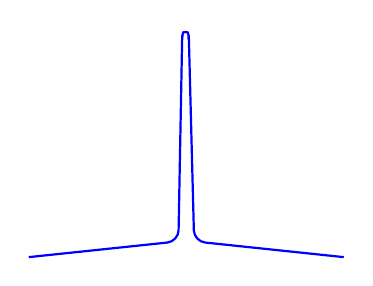
\begin{tikzpicture}
\YEaaxis{1}{4}{1}{3}
\YExcoord{1}{a}
\YExcoord{2}{}
\YExcoord{3}{b}
\draw[thick, blue, rounded corners] (0,.1)--(1.9,.3)--(1.95,3) arc(180:360:.4mm)-- (2.1,.3)--(4,.1);
\end{tikzpicture}
\end{center}

The trapezoidal approximation of $\displaystyle\int_a^b f(x)~\dee{x}$ with $n=1$ misses the thin spike, and gives a mild underapproximation. By contrast, the midpoint approximation with $n=1$ takes the spike as the height of the entire region, giving a vast overapproximation.

\begin{center}
\begin{tikzpicture}
\draw[thick, red, fill=red, fill opacity=0.2] (1,.2) rectangle (3,0);

\YEaaxis{1}{4}{1}{3}
\YExcoord{1}{a}
\YExcoord{2}{}
\YExcoord{3}{b}
\draw[thick, blue, rounded corners] (0,.1)--(1.9,.3)--(1.95,3) arc(180:360:.4mm)-- (2.1,.3)--(4,.1);
\draw[red] (1,.2) node[vertex]{};
\draw[red] (3,.2) node[vertex]{};
\draw (2,-1) node {trapezoidal};
\end{tikzpicture}
\hspace{2cm}
\begin{tikzpicture}
\draw[red, thick, fill=red, fill opacity=0.2] (1,3) rectangle (3,0);

\YEaaxis{1}{4}{1}{3}
\YExcoord{1}{a}
\YExcoord{2}{}
\YExcoord{3}{b}
\draw[thick, blue, rounded corners] (0,.1)--(1.9,.3)--(1.95,3) arc(180:360:.4mm)-- (2.1,.3)--(4,.1);
\draw[red] (2,3) node[vertex]{};
\draw (2,-1) node {midpoint};
\end{tikzpicture}
\end{center}

\end{solution}
%%%%%%%%%%%%%%%%%%%



\begin{Mquestion}[2015A]
Decide whether the following statement is true or false.
If false, provide a counterexample. If true, provide a brief justification.

\begin{quote}\color{blue}
When $f(x)$ is positive and concave up, any trapezoidal rule approximation for $\displaystyle\int_{a}^{b} f(x) \,\dee{x}$ will be an upper estimate for $\displaystyle\int_{a}^{b} f(x) \,\dee{x}$.
\end{quote}
\end{Mquestion}

\begin{hint}
Draw a sketch.
\end{hint}

\begin{answer}
True. Because $f(x)$ is positive and concave up,
the graph of $f(x)$ is always below the top edges of the trapezoids
used in the trapezoidal rule.

\begin{center}
\begin{tikzpicture}
\YEaaxis{3}{3}{1}{3}
\draw[thick, blue] plot[domain=-3:3](\x,{\x*\x/4+.5}) node[right]{$y=f(x)$};
\draw[red] (-1,.75) node[vertex](a){};
\draw[red] (2,1.5) node[vertex](b){};
\filldraw[red, thick, fill opacity=0.1] (-1,.75)|-(2,0)--(2,1.5)--(-1,.75);
\end{tikzpicture}
\end{center}
\end{answer}

\begin{solution}
True. Because $f(x)$ is positive and concave up,
the graph of $f(x)$ is always below the top edges of the trapezoids
used in the trapezoidal rule.

\begin{center}
\begin{tikzpicture}
\YEaaxis{3}{3}{1}{3}
\draw[thick, blue] plot[domain=-3:3](\x,{\x*\x/4+.5}) node[right]{$y=f(x)$};
\draw[red] (-1,.75) node[vertex](a){};
\draw[red] (2,1.5) node[vertex](b){};
\filldraw[red, thick, fill opacity=0.1] (-1,.75)|-(2,0)--(2,1.5)--(-1,.75);
\end{tikzpicture}
\end{center}
\end{solution}
%%%%%%%%%%%%%%%%%%%

\begin{question}
Give a polynomial $f(x)$ with the property that
 the Simpson's rule approximation of $\displaystyle\int_a^b f(x)~\dee{x}$ is exact for all $a$, $b$, and $n$.
\end{question}
\begin{hint}
The error bound for the approximation is given in Theorem~\eref{CLP101}{thm num int err} in the CLP-2 text. You want this bound to be zero.
\end{hint}
\begin{answer}
Any polynomial of degree at most 3 will do. For example, $f(x)=5x^3-27$, or $f(x)=x^2$.
\end{answer}
\begin{solution}
According to Theorem~\eref{CLP101}{thm num int err}  in the CLP-2 text, the error associated with the Simpson's rule approximation is no more than $\dfrac{L}{180}\dfrac{(b-a)^5}{n^4}$, where $L$ is a constant such that $|f^{(4)}(x)| \leq L$ for all $x$ in $[a,b]$. If $L=0$, then the error is no more than 0 regardless of $a$, $b$, or $n$--that is, the approximation is exact.

Any polynomial $f(x)$ of degree at most 3 has $f^{(4)}(x)=0$ for all $x$. So, any polynomial of degree at most 3 is an acceptable answer. For example, $f(x)=5x^3-27$, or $f(x)=x^2$.
\end{solution}
%%%%%%%%%%%%%%%%%%%



%%%%%%%%%%%%%%%%%%
\subsection*{\Procedural}
%%%%%%%%%%%%%%%%%%
\Instructions{Questions
\ref{prob_s1.11_int1} and \ref{prob_s1.11_int2}
ask you to approximate a given integral  using the formulas in Equations~\eref{CLP101}{eq:MPrule},
\eref{CLP101}{eq:TRPrule}, and \eref{CLP101}{eq:SIMPrule} in the CLP-2 text.}
\begin{Mquestion}\label{prob_s1.11_int1}
Write out all three approximations of $\displaystyle\int_0^{30} \frac{1}{x^3+1}~\dee{x}$ with $n=6$. (That is: midpoint, trapezoidal, and Simpson's.) You do not need to simplify your answers.
\end{Mquestion}
\begin{hint}
Follow the formulas in Equations~\eref{CLP101}{eq:MPrule},
\eref{CLP101}{eq:TRPrule}, and \eref{CLP101}{eq:SIMPrule} in the CLP-2 text.
\end{hint}
\begin{answer}

Midpoint:\\[10pt]
$\displaystyle
\int_0^{30} \frac{1}{x^3+1}\,\dee{x}\approx\left[\tfrac{1}{\left(2.5\right)^3+1}
+\tfrac{1}{\left(7.5\right)^3+1}
+\tfrac{1}{\left(12.5\right)^3+1}
+\tfrac{1}{\left(17.5\right)^3+1}
+\tfrac{1}{\left(22.5\right)^3+1}
+\tfrac{1}{\left(27.5\right)^3+1}
\right]5
$

Trapezoidal:\\[10pt]
$\displaystyle\int_0^{30} \frac{1}{x^3+1}\,\dee{x}
\approx\left[
\frac{1/2}{0^3+1}+
\frac{1}{5^3+1}+
\frac{1}{10^3+1}+
\frac{1}{15^3+1}+
\frac{1}{20^3+1}+
\frac{1}{25^3+1}+
\frac{1/2}{30^3+1}
\right]5$

Simpson's:\\[10pt]
$
\displaystyle\int_0^{30} \frac{1}{x^3+1}\,\dee{x}\approx
\Big[\frac{1}{{0}^3+1}\!+\frac{4}{{5}^3+1}\!+\frac{2}{{10}^3+1}\!+\frac{4}{{15}^3+1}\!+\frac{2}{{20}^3+1}\!+\frac{4}{{25}^3+1}\!+ \frac{1}{{30}^3+1}\Big]\frac{5}{3}
$
\end{answer}
\begin{solution}
\begin{itemize}
\item For all three approximations, $\Delta x = \dfrac{b-a}{n}=\dfrac{30-0}{6}=5$.


\item For the trapezoidal rule and Simpson's rule, the $x$-values where we evaluate $\dfrac{1}{x^3+1}$ start at $x=a=0$ and move up by $\Delta x = 5$:  $x_0=0$, $x_1=5$,
 $x_2=10$, $x_3=15$,
  $x_4=20$, $x_5=25$, and $x_6=30$.

  \begin{center}
  \begin{tikzpicture}[scale=1.8]
  \draw[<->, thick] (-1,0)--(7,0);
  \foreach \x in {0,...,6}{
  	\MULTIPLY{\x}{5}{\l}
	\YExcoord{\x}{\atp{\l}{x_{\x}}}}
  \end{tikzpicture}
  \end{center}

\item For the midpoint rule, the $x$-values where we evaluate $\dfrac{1}{x^3+1}$ start at $x=2.5 = \frac{x_0+x_1}{2}$ and move up by $\Delta x = 5$:  $\bar x_1=2.5$, $\bar x_2=7.5$,
 $\bar x_3=12.5$, $\bar x_4=17.5$,
  $\bar x_5=22.5$, and $\bar x_6=27.5$.


  \begin{center}
  \begin{tikzpicture}[scale=1.8]
  \draw[<->, thick] (-1,0)--(7,0);
  \foreach \x in {0,...,6}{
  	\MULTIPLY{\x}{5}{\l}
	\color{gray}
	\YExcoord{\x}{\atp{\l}{x_{\x}}}
	\ADD{\x}{.5}{\y};
	\ADD{\l}{2.5}{\m}}
  \foreach \x in {1,...,6}{
  	\MULTIPLY{\x}{5}{\l}
	\SUBTRACT{\x}{.5}{\y};
	\SUBTRACT{\l}{2.5}{\m}
	\color{red}
	\YExcoord{\y}{\atp{\m}{\bar x_{\x}}}}

  \end{tikzpicture}
  \end{center}

\item  Following Equation~\eref{CLP101}{eq:MPrule} in the CLP-2 text,
the midpoint rule approximation is:
\begin{align*}
\int_0^{30} \frac{1}{x^3+1}\,\dee{x}&\approx\Big[f(\bar x_1)+f(\bar x_2)+\cdots
+f(\bar x_n)\Big]\De x\\
&=\left[\tfrac{1}{\left(2.5\right)^3+1}
+\tfrac{1}{\left(7.5\right)^3+1}
+\tfrac{1}{\left(12.5\right)^3+1}
+\tfrac{1}{\left(17.5\right)^3+1}
+\tfrac{1}{\left(22.5\right)^3+1}
+\tfrac{1}{\left(27.5\right)^3+1}
\right]5
\end{align*}

 \item
  Following Equation~\eref{CLP101}{eq:TRPrule} in the CLP-2 text, the trapezoidal rule approximation is:
\begin{align*}
\int_0^{30} \frac{1}{x^3+1}\,\dee{x}
&\approx\Big[\half f(x_0)+f(x_1)+f(x_2)+\cdots+ f(x_{n-1})+\half f(x_n)\Big]\De x\\
&=\left[
\frac{1/2}{0^3+1}+
\frac{1}{5^3+1}+
\frac{1}{10^3+1}+
\frac{1}{15^3+1}+
\frac{1}{20^3+1}+
\frac{1}{25^3+1}+
\frac{1/2}{30^3+1}
\right]5
\end{align*}

\item Following Equation~\eref{CLP101}{eq:SIMPrule} in the CLP-2 text, the Simpson's rule approximation is:
\begin{align*}
\int_0^{30} \frac{1}{x^3+1}\,\dee{x}
&\approx\Big[f(x_0)\!+4f(x_1)\!+2f(x_2)\!+4f(x_3)\!+2f(x_4)\!+4f(x_{5})\!+ f(x_6)\Big]\tfrac{\De x}{3}\\
&=\Big[\frac{1}{{0}^3+1}\!+\frac{4}{{5}^3+1}\!+\frac{2}{{10}^3+1}\!+\frac{4}{{15}^3+1}\!+\frac{2}{{20}^3+1}\!+\frac{4}{{25}^3+1}\!+ \frac{1}{{30}^3+1}\Big]\frac{5}{3}
\end{align*}

\end{itemize}
\end{solution}
%%%%%%%%%%%%%%%%%%%


\begin{question}[M121 2012A]\label{prob_s1.11_int2}
Find the midpoint rule approximation to $\displaystyle\int_0^\pi \sin x\ \dee{x}$
with $n = 3$.
\end{question}

\begin{hint}
See Section~\eref{CLP101}{sec:midpointRule} in the
%\href{http://www.math.ubc.ca/%7Efeldman/m101/clp/clp_notes_101.pdf}{CLP-2 text}.
CLP-2 text. You should be able to simplify your answer to an exact value (in terms of $\pi$).
\end{hint}

\begin{answer}
$\dfrac{2\pi}{3}$
\end{answer}

\begin{solution}
By Equation~\eref{CLP101}{eq:MPrule} in the CLP-2 text,
the midpoint rule approximation
to $\int_a^b f(x)\ \dee{x}$ with $n=3$ is
\begin{align*}
\int_a^b f(x)\,\dee{x}\approx\big[f(\bar x_1)+f(\bar x_2)+f(\bar x_3)\big]\De x
\end{align*}
where $\De x = \tfrac{b-a}{3}$ and
\begin{alignat*}{7}
x_0&=a&\quad
x_1&=a+\De x&\quad
x_2&=a+2\De x&\quad
x_3&=b\\
& &
\bar x_1&=\tfrac{x_0+x_1}{2}&
\bar x_2&=\tfrac{x_1+x_2}{2}&
\bar x_3&=\tfrac{x_2+x_3}{2}
\end{alignat*}
For this problem, $a=0$, $b=\pi$ and $f(x) = \sin x$, so that
$\De x = \tfrac{\pi}{3}$  and
\begin{alignat*}{7}
x_0&=0&\quad
x_1&=\tfrac{\pi}{3}&\quad
x_2&=\tfrac{2\pi}{3}&\quad
x_3&=\pi\\
& &
\bar x_1&=\tfrac{\pi}{6}&
\bar x_2&=\tfrac{\pi}{2}&
\bar x_3&=\tfrac{5\pi}{6}
\end{alignat*}



  \begin{center}
  \begin{tikzpicture}[scale=1.8]
  \draw[<->, thick] (-1,0)--(7,0);
	\YExcoord{0}{\atp{0}{x_{0}}}
	\YExcoord{6}{\atp{\pi}{x_{3}}}
	\YExcoord{2}{\atp{\pi/3}{x_{1}}}
	\YExcoord{4}{\atp{2\pi/3}{x_{2}}}
\color{red}
	\YExcoord{1}{\atp{\pi/6}{\bar x_{1}}}
	\YExcoord{3}{\atp{\pi/2}{\bar x_{2}}}
	\YExcoord{5}{\atp{5\pi/6}{\bar x_{3}}}
  \end{tikzpicture}
  \end{center}


Therefore,
\begin{align*}
\int_0^\pi \sin x\ \dee{x}
&\approx\left[\sin\frac{\pi}{6}
            +\sin \frac{\pi}{2}
            +\sin \frac{5\pi}{6}\right]\frac{\pi}{3}
=\left[\frac{1}{2}
            +1
            +\frac{1}{2}\right]\frac{\pi}{3}
=\frac{2\pi}{3}
\end{align*}

\end{solution}
%%%%%%%%%%%%%%%%%%%
\Instructions{Questions~\ref{prob_s1.11_tableproblem1} though
\ref{prob_s1.11_tableproblem3}
ask you to approximate a quantity based on observed data.}
%%%%%%%%%%%%%%%%%%%


\begin{question}[1997D]\label{prob_s1.11_tableproblem1}
The solid $V$ is 40 cm high and the horizontal cross sections
are circular disks. The table below gives the diameters of the cross sections
in centimeters at 10 cm intervals. Use the trapezoidal rule to estimate
the volume of $V$.

\renewcommand{\arraystretch}{1.1}
\begin{center}
     \begin{tabular}{|l|c|c|c|c|c|}
          \hline
          height&0&10&20&30&40  \\
          \hline
          diameter&24&16&10&6&4 \\
          \hline
     \end{tabular}
\end{center}
\renewcommand{\arraystretch}{1.0}
\end{question}

\begin{hint}
See Section~\eref{CLP101}{sec:trapRule} in the
%\href{http://www.math.ubc.ca/%7Efeldman/m101/clp/clp_notes_101.pdf}{CLP-2 text}.
CLP-2 text.
To set up the volume integral, see Example \eref{CLP101}{eg:VOLb} in the
%\href{http://www.math.ubc.ca/%7Efeldman/m101/clp/clp_notes_101.pdf}{CLP-2 text}.
CLP-2 text. Note the dimensions given for the cross sections are diameters, not radii.
\end{hint}

\begin{answer}
$1720\pi\approx 5403.5\ {\rm cm}^3$
\end{answer}

\begin{solution}
Let $f(x)$ denote the diameter at height $x$.
As in Example \eref{CLP101}{eg:VOLb} of the
%\href{http://www.math.ubc.ca/%7Efeldman/m101/clp/clp_notes_101.pdf}{CLP-2 text}.
CLP-2 text, we slice $V$  into thin horizontal ``pancakes'', which in
this case are circular.

\begin{center}
\begin{tikzpicture}
\draw plot[domain=0:4]({(\x*\x+\x+4)/6} ,4-\x);
\draw plot[domain=0:4]({1-(\x*\x+\x+4)/6} ,4-\x);
\draw (.6667,4) arc(0:360:1.667mm and 0.666 mm);
\draw (-3,0) arc (180:360:35mm and 7mm);
\draw[dashed] (-2.95,0) arc (170:10:35mm and 7mm);
%\draw (-1,0) grid[] (4,4);
\draw (.5,3) node[shape=ellipse, minimum width=1cm, minimum height=2mm, fill, fill opacity=0.2, draw]{};
\filldraw[fill opacity=0.3] (0,3)--(0,2.8) arc (180:360: .5cm and 2mm)--(1,3) arc (0:-180: .5cm and 2mm);
\draw (-1,2.95) node[left]{$\dee{x}$};
\draw (-.7,2.8)-|(-.9,3.0) --(-.7,3.0);
\draw[|-|] (0,2.25)--(1,2.25) node[midway, below]{$f(x)$};
\draw[help lines, <->] (-4,-.5)--(-4,4.5) node[above]{$x$};
\end{tikzpicture}
\end{center}

\begin{itemize}
\item We are told that the pancake at height $x$ is a circular disk
of diameter $f(x)$ and so
\item has cross-sectional area $\pi\big(\frac{f(x)}{2}\big)^2$ and
thickness $\dee{x}$ and hence
\item has volume $\pi\big(\frac{f(x)}{2}\big)^2\dee{x}$.
\end{itemize}


\noindent Hence the volume of $V$ is
\begin{align*}
\int_0^{40}\pi\Big{[\frac{f(x)}{2}\Big]}^2\,\dee{x}
&\approx \frac{\pi}{4}10\Big[\half f(0)^2+f(10)^2+f(20)^2+f(30)^2+\half
f(40)^2\Big]\\
&=\frac{\pi}{4}10\Big[\half 24^2+16^2+10^2+6^2+\half 4^2\Big]\\
&=688\times 2.5\pi
=1720\pi\approx 5403.5
\end{align*}
where we have approximated the integral using the trapezoidal rule with $\De
x=10$, and used a calculator to get a decimal approximation.


\end{solution}
%%%%%%%%%%%%%%%%%%%
\begin{question}[1996D]\label{prob_s1.11tableproblem2}
A $6$ metre long cedar log has cross sections that are approximately
circular. The diameters of the log, measured at one metre intervals, are
given below:

\renewcommand{\arraystretch}{1.1}
\begin{center}
     \begin{tabular}{|l|c|c|c|c|c|c|c|}
          \hline
          metres from left end of log&0&1&2&3&4&5&6  \\
          \hline
          diameter in metres         &1.2&1&0.8&0.8&1&1&1.2 \\
          \hline
     \end{tabular}
\end{center}
\renewcommand{\arraystretch}{1.0}

\noindent Use Simpson's Rule to estimate the volume of the log.

\end{question}

\begin{hint}
See Section \eref{CLP101}{sec:Simpson} in the
%\href{http://www.math.ubc.ca/%7Efeldman/m101/clp/clp_notes_101.pdf}{CLP-2 text}.
CLP-2 text, and compare to Question~\ref{prob_s1.11_tableproblem1}. Note the table gives diameters, not radii.
\end{hint}

\begin{answer}
$\displaystyle\frac{\pi}{12}(16.72)\approx4.377\ {\rm m}^3$
\end{answer}

\begin{solution}
 Let $f(x)$ be the diameter a distance $x$ from the left end of
the log.
If we slice our log into thin disks, the disks $x$ metres from the left end of the log has
\begin{itemize}
\item radius $\frac{f(x)}{2}$,
\item width $\dee{x}$, and so
\item volume $\pi\left(\frac{f(x)}{2}\right)^2~\dee{x}=\frac{\pi}{4}f(x)^2~\dee{x}$.
\end{itemize}

\begin{center}
\begin{tikzpicture}
\draw plot[domain=0:3.14]({3*\x},{-sin(\x r)/3});
\draw plot[domain=0:3.14]({3*\x},{-2+sin(\x r)/3});
\draw(0,-2) arc(270:90: 2.5mm and 1cm);
\draw[dashed](0,-2) arc(270:-270: 2.5mm and 1cm);
\draw (9.42,-1) node[shape=ellipse, minimum height=2cm, minimum width=5mm, draw]{};
\draw[] (4.71,-1) node[shape=ellipse, minimum height=1.33cm, minimum width=4mm, draw, fill, fill opacity=0.1]{};
\filldraw[fill opacity=0.3] (4.71,-.33) -- (4.51,-.33 )arc (90:270:2mm and 6.67mm) --(4.71,-1.67)
arc (270:90:2mm and 6.67mm) ;
\draw[<->, help lines] (-1,-3)--(11,-3) node[right]{$x$};
\draw[|-|] (3.5,-.4)--(3.5,-1.6) node[midway, left]{$f(x)$};
\draw[|-|] (4.5,0)--(4.7,0) node[above, midway]{$\dee{x}$};
\end{tikzpicture}
\end{center}

Using Simpson's Rule with $\De
x=1$,
the volume
of the log is:
\begin{align*}
V=\int_0^6 \frac{\pi}{4}f(x)^2\,\dee{x}
&\approx\frac{\pi}{4}\frac{1}{3}
\Big[f(0)^2+4f(1)^2+2f(2)^2+4f(3)^2+2f(4)^2+4f(5)^2+f(6)^2\Big]\\
&=\frac{\pi}{12}
\Big[1.2^2+4(1)^2+2(0.8)^2+4(0.8)^2+2(1)^2+4(1)^2+1.2^2\Big]\\
&=\frac{\pi}{12}(16.72)\\
&\approx4.377\ {\rm m}^3
\end{align*}
where we used a calculator to approximate the decimal value.
\end{solution}
%%%%%%%%%%%%%%%%%%%

\begin{question}[1998A]
 The circumference of an 8 metre high tree at different heights
above the ground is given in the table below. Assume that all horizontal
cross-sections of the tree are circular disks.

\renewcommand{\arraystretch}{1.1}
\begin{center}
     \begin{tabular}{|l|c|c|c|c|c|}
          \hline
          height (metres) &0&2&4&6&8  \\
          \hline
          circumference (metres) &1.2&1.1&1.3&0.9&0.2\\
          \hline
     \end{tabular}
\end{center}
\renewcommand{\arraystretch}{1.0}

\noindent Use Simpson's rule to approximate the volume of the tree.
\end{question}

\begin{hint}
See \S\eref{CLP101}{sec:Simpson} in the
%\href{http://www.math.ubc.ca/%7Efeldman/m101/clp/clp_notes_101.pdf}{CLP-2 text}.
CLP-2 text.
To set up the volume integral, see Example \eref{CLP101}{eg:VOLb} in the
%\href{http://www.math.ubc.ca/%7Efeldman/m101/clp/clp_notes_101.pdf}{CLP-2 text}.
CLP-2 text, or Question~\ref{prob_s1.11tableproblem2}.

Note that the table gives the circumference, not radius, of the tree at a given height.
\end{hint}

\begin{answer}
$\dfrac{12.94}{6\pi}
\approx0.6865\ {\rm m}^3$
\end{answer}

\begin{solution}
At height $x$ metres, let the circumference of the tree be $c(x)$.
The corresponding
radius is $\dfrac{c(x)}{2\pi}$, so the corresponding cross-sectional area
is $\pi\left(\dfrac{c(x)}{2\pi}\right)^2=\dfrac{c(x)^2}{4\pi}$.


\begin{center}
\begin{tikzpicture}
\draw[thick, rounded corners](3,0)--(2.75,2)--(3.25,4)--(2.25,6)--(.5,8);
\draw[thick, rounded corners](-3,0)--(-2.75,2)--(-3.25,4)--(-2.25,6)--(-.5,8);
\draw (0,8) node[shape=ellipse, minimum width = 1cm, minimum height=1mm, draw]{};
\draw (-3,0) arc (180:360:3cm and 3mm);
\draw (0,6) node[shape=ellipse, minimum width = 4.5cm, minimum height=5.5mm, draw, fill, fill opacity=0.2]{};
\draw (-2.25,6)--(-2.25,5.5) arc (180:360:2.25cm and 2.75mm) --(2.25,6);
\draw[|-|] (-2.75,6)--(-2.75,5.5) node[midway, left]{$\dee{x}$};
\draw[ <->] (0,3.5)+(135:2.25cm) arc(135:405: 2.25cm and 2.75mm) node[midway, below]{$c(x)$};
\draw[help lines, <->] (-4,-.5) --(-4,9) node[above]{$x$};
\end{tikzpicture}
\end{center}

The height of a very thin cross-sectional  disk is $\dee{x}$, so the
volume of a cross-sectional disk is $\dfrac{c(x)^2}{4\pi}~\dee{x}$.
Therefore,
total volume of the tree is:
\begin{align*}
\int_0^8 \frac{c(x)^2}{4\pi}\,\dee{x}
&\approx \frac{1}{4\pi}\frac{2}{3}\Big[c(0)^2+4c(2)^2+2c(4)^2+4c(6)^2+c(8)^2\Big]\cr
&=\frac{1}{6\pi}\Big[1.2^2+4(1.1)^2+2(1.3)^2+4(0.9)^2+0.2^2\Big]\\
&=\frac{12.94}{6\pi}
\approx0.6865
\end{align*}
where we used Simpson's rule with $\De x = 2$ and $n=4$ to approximate the value of the integral based on the values of $c(x)$ given in  the table.
\end{solution}
%%%%%%%%%%%%%%%%%%%

\begin{Mquestion}[2001A]
By measuring the areas enclosed by contours on a topographic map, a geologist
determines the cross sectional areas $A$ in $\mathrm{m}^2$ of a $60$ m high
hill. The table below gives the cross sectional area $A(h)$ at various
heights $h$. The volume of the hill is $V=\int_0^{60} A(h)\,\dee{h}$.

\renewcommand{\arraystretch}{1.1}
\begin{center}
     \begin{tabular}{|l|c|c|c|c|c|c|c|}
          \hline
          $h$ &0&10&20&30&40&50&60  \\
          \hline
          $A$ &10,200&9,200&8,000&7,100&4,500&2,400&100\\
          \hline
     \end{tabular}
\end{center}
\renewcommand{\arraystretch}{1.0}

\begin{enumerate}[(a)]
\item
If the geologist uses the Trapezoidal Rule to estimate the
volume of the hill, what will be their estimate, to the nearest 1,000$\mathrm{m}^3$?
\item
What will be the geologist's estimate of the volume of the
hill if they use Simpson's Rule instead of the Trapezoidal Rule?
\end{enumerate}
\end{Mquestion}

\begin{answer}
(a) 363,500
\qquad (b) 367,000
\end{answer}

\begin{solution}
For both approximations, $\De x = 10$ and $n=6$.

 (a)
The Trapezoidal Rule gives
\begin{align*}
V&=\int_0^{60} A(h)\,\dee{h}
\approx 10\Big[\half A(0)+A(10)+A(20)+A(30)+A(40)+A(50)+\half A(60)\Big] \\
&=\text{363,500}
\end{align*}

\noindent (b)
Simpson's Rule gives
\begin{align*}
V&=\int_0^{60} A(h)\,\dee{h}
\approx \frac{10}{3}\Big[A(0)+4A(10)+2A(20)+4A(30)+2A(40)+4A(50)+A(60)\Big]\\
&=\text{367,000}
\end{align*}

\end{solution}
%%%%%%%%%%%%%%%%%%%%%%%%%%%%%%%%%%%%%%%%


\begin{Mquestion}[2013A]\label{prob_s1.11_tableproblem3}
The graph below applies to both parts (a) and (b).

\begin{center}
       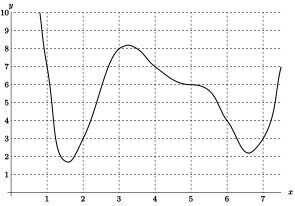
\includegraphics{OE13A_1}
\end{center}


\begin{enumerate}[(a)]
\item
Use the Trapezoidal Rule, with $n = 4$, to estimate
the area under the graph between $x = 2$ and $x = 6$.
Simplify your answer completely.
\item
Use Simpson's Rule, with $n = 4$, to estimate the
area under the graph between $x = 2$ and $x = 6$.
\end{enumerate}
\end{Mquestion}

\begin{answer}
(a) $\dfrac{49}{2}$
\qquad (b) $\dfrac{77}{3}$
\end{answer}

\begin{solution}
Call the curve in the graph $y=f(x)$. It looks like
\begin{align*}
f(2)=3 \qquad
f(3)=8 \qquad
f(4)=7 \qquad
f(5)=6 \qquad
f(6)=4
\end{align*}

We're estimating $\int_2^6 f(x)~\dee{x}$ with $n=4$, so $\De x = \frac{6-2}{4}=1$.

\noindent (a)
The trapezoidal rule gives
\begin{align*}
T_4=\left[\frac{3}{2}+ 8+7+ 6+\frac{4}{2}\right]\times 1=\frac{49}{2}
\end{align*}

\noindent (b)
Simpson's rule gives
\begin{align*}
S_4=\frac{1}{3}\big[3+4\times 8+2\times 7+4\times 6+4\big]\times 1
=\frac{77}{3}
\end{align*}

\end{solution}
%%%%%%%%%%%%%%%%%%%%%%%%%%%%%%%%%%%%%%%%

\Instructions{In Questions~\ref{prob_s.1.11_error1} through \ref{prob_s.1.11_error2}, we practice finding error bounds for our approximations.}

\begin{question}[2016Q4]\label{prob_s.1.11_error1}
The integral $\displaystyle\int_{-1}^{1} \sin(x^2) \, \dee{x}$ is estimated using the Midpoint
Rule with $1000$ intervals.  Show that the absolute error in this approximation is at most
$2\cdot 10^{-6}$.

You may use the fact that when approximating $\int_a^b f(x) \, \dee{x}$ with the
Midpoint Rule using $n$ points, the absolute value
of the error is at most $M(b-a)^3/24n^2$ when $\left|f''(x)\right|\leq M$
for all $x\in[a,b]$.
\end{question}

\begin{hint}
The main step is to find an appropriate value of $M$. It is \emph{not necessary} to
find the smallest possible $M$.
\end{hint}

\begin{answer}
Let $f(x) = \sin(x^2)$.  Then $f'(x) = 2x \cos(x^2)$ and
$$f''(x) = 2\cos(x^2) - 4x^2\sin(x^2).$$
Since $|x^2|\le1$ when $|x|\leq 1$, and $\left|\sin\theta\right|\le1$ and $\left|\cos\theta\right|\leq 1$ for all $\theta$,
we have
\begin{align*}
\left|2\cos(x^2) - 4x^2\sin(x^2)\right|
\le 2|\cos(x^2)| +  4x^2|\sin(x^2)|
\le 2\times 1 +4\times 1\times 1
= 2+4 = 6
\end{align*}
We can therefore choose $M=6$, and it follows that the error is at most \begin{align*}
\frac{M[b-a]^3}{24n^2}
\le \frac{6\cdot [1-(-1)]^3}{24 \cdot 1000^2}
= \frac{2}{10^6}  = 2\cdot 10^{-6}
\end{align*}\end{answer}

\begin{solution}
Let $f(x) = \sin(x^2)$.  Then $f'(x) = 2x \cos(x^2)$ and
$$f''(x) = 2\cos(x^2) - 4x^2\sin(x^2).$$
Since $|x^2|\le1$ when $|x|\leq 1$, and $\left|\sin\theta\right|\le1$ and $\left|\cos\theta\right|\leq 1$ for all $\theta$,
we have
\begin{align*}
\left|2\cos(x^2) - 4x^2\sin(x^2)\right|
\le 2|\cos(x^2)| +  4x^2|\sin(x^2)|
\le 2\times 1 +4\times 1\times 1
= 2+4 = 6
\end{align*}
We can therefore choose $M=6$, and it follows that the error is at most \begin{align*}
\frac{M[b-a]^3}{24n^2}
\le \frac{6\cdot [1-(-1)]^3}{24 \cdot 1000^2}
= \frac{2}{10^6}  = 2\cdot 10^{-6}
\end{align*}
\end{solution}
%%%%%%%%%%%%%%%%%%%


\begin{Mquestion}[2016Q4]
The total error using the midpoint rule with $n$ subintervals to
approximate the integral of $f(x)$ over $[a,b]$ is bounded by
$\dfrac{M (b-a)^3}{(24n^2)}$, if $|f''(x)| \le M$ for all  $a \le x \le b$.

Using this bound, if the integral $\displaystyle\int_{-2}^{1} 2x^4 \,\dee{x}$ is approximated using the midpoint rule with $60$ subintervals, what is the largest possible error between the approximation $M_{60}$ and the true value of the integral?
\end{Mquestion}

\begin{hint}
The main step is to find $M$. This question is unusual in that its
wording requires you to find the smallest possible allowed $M$.
\end{hint}

\begin{answer}
$\dfrac{3}{100}$
\end{answer}

\begin{solution}
Setting $f(x) = 2 x^4$ and $b-a = 1-(-2)=3$, we compute $f''(x) = 24x^2$.
The largest value of $24x^2$ on the interval $[-2,1]$ occurs at $x=-2$,
so we can take $M = 24\cdot(-2)^2=96$. Thus the total error for the midpoint rule with $n=60$ points is bounded by
\begin{align*}
\frac{M (b-a)^3}{24n^2}  = \frac{96 \times 3^3}{24 \times 60 \times 60} = \frac{3}{100}
\end{align*}

That is: we are guaranteed our absolute error is certainly no more\footnote{This is what the error bound always tells us.} than $\frac{3}{100}$, and using the bound stated in the problem we cannot give a better guarantee.
(The second part of the previous sentence comes from the fact that we used the smallest possible $M$: if we had used a larger value of $M$, we would still have some true statement about the error, for example ``the error is no more than $\frac{5}{100}$," but it would not be the
\emph{best} true statement we could make.)
\end{solution}
%%%%%%%%%%%%%%%%%%%%%%%%%%%%%%%%%%%%%%%%%%%%%%%

\begin{question}[2016A]
Both parts of this question concern the integral $I = \displaystyle\int_{0}^{2} (x-3)^5\,\dee{x}$.
\begin{enumerate}[(a)]
\item
Write down the Simpson's Rule approximation to $I$ with $n=6$.
Leave your answer in calculator-ready form.

\item
Which method of approximating $I$ results in a smaller error bound:
the Midpoint Rule with $n=100$ intervals, or Simpson's Rule with $n=10$
intervals?  You may use the formulas
\begin{align*}
|E_M| \le \frac{M(b-a)^3}{24n^2} \qquad\text{and}\qquad |E_S| \le \frac{L(b-a)^5}{180n^4},
\end{align*}
where $M$ is an upper bound for $|f''(x)|$ and $L$ is an upper bound for $|f^{(4)}(x)|$, and $E_M$ and $E_S$ are the absolute errors arising from the midpoint rule and Simpson's rule, respectively.
\end{enumerate}
\end{question}

\begin{hint}
The main steps in part (b) are to find the smallest possible values of
$M$ and $L$.
\end{hint}

\begin{answer}
(a) $\dfrac{1/3}3 \Big( (-3)^5 + 4\Big( \frac13-3 \Big)^5 + 2\Big( \frac23-3 \Big)^5 + 4(-2)^5 + 2\Big( \frac43-3 \Big)^5 + 4\Big( \frac53-3 \Big)^5 + (-1)^5 \Big)$

\noindent (b)
Simpson's Rule results in a smaller error bound.
\end{answer}

\begin{solution} (a)
Since $a=0$, $b=2$ and $n=6$, we have
   $\Delta x=\frac{b-a}{n}=\frac{2-0}6 = \frac{1}{3}$,
and so $x_0=0$, $x_1=\frac{1}{3}$, $x_2=\frac{2}{3}$, $x_3=1$,
$x_4=\frac{4}{3}$, $x_5=\frac{5}{3}$, and $x_6=2$. Since Simpson's
Rule with $n=6$ in general is
\begin{align*}
\frac{\Delta x}3 \big[ f(x_0) + 4f(x_1) + 2f(x_2) + 4f(x_3) + 2f(x_4) + 4f(x_5) + f(x_6) \big],
\end{align*}
the desired approximation is
\begin{align*}
\frac{1/3}3 \bigg( (-3)^5 + 4\Big( \frac13-3 \Big)^5 + 2\Big( \frac23-3 \Big)^5 + 4(-2)^5 + 2\Big( \frac43-3 \Big)^5 + 4\Big( \frac53-3 \Big)^5 + (-1)^5 \bigg)
\end{align*}

\noindent (b)
Here $f(x) = (x-3)^5$, which has derivatives
\begin{align*}
f'(x) &= 5(x-3)^4 & f''(x) &= 20(x-3)^3 \\
f^{(3)}(x) &= 60(x-3)^2 & f^{(4)}(x) &= 120(x-3).
\end{align*}
For $0\le x\le 2$, $(x-3)$ runs from $-3$ to $-1$, so the maximum
absolute values are found at $x=0$, giving
$M= 20\cdot|0-3|^3=540$ and $L=120\cdot|0-3|=360$. Consequently, for
the Midpoint Rule with $n=100$,
\begin{align*}
|E_M| \le \frac{M(b-a)^3}{24n^2} = \frac{540 \times 2^3}{24 \times 10^4} = \frac{180}{10^4};
\end{align*}
whereas for Simpson's Rule with $n=10$,
\begin{align*}
|E_S| \le \frac{360 \times 2^5 }{180 \times 10^4}  = \frac{64}{10^4}.
\end{align*}
Since $64<180$, Simpson's Rule results in a smaller error bound.

\end{solution}
%%%%%%%%%%%%%%%%%%%%%%%%%%%%%%%%


\begin{question}[M105 2013A]
Find a bound for the error in approximating
$\displaystyle\int_1^5 \frac{1}{x}\,\dee{x}$ using Simpson's rule with $n = 4$.
Do not write down the Simpson's rule approximation $S_4$.

In general the error in approximating
$\int_a^b f(x)\ \dee{x}$ using Simpson's rule with $n$
steps is bounded by $\dfrac{L(b-a)}{180}(\De x)^4$ where $\De x=\dfrac{b-a}{n}$
and $L\ge |f^{(4)}(x)|$ for all $a\le x\le b$.
\end{question}

\begin{hint}
As usual, the biggest part of this problem is finding $L$. Don't be thrown off by the error bound being given slightly differently from Theorem~\eref{CLP101}{thm num int err} in the CLP-2 text: these expressions are equivalent, since $\De x = \frac{b-a}{n}$.
\end{hint}

\begin{answer}
$\dfrac{8}{15}$
\end{answer}

\begin{solution}
In general the error in approximating
$\int_a^b f(x)\ \dee{x}$ using Simpson's rule with $n$
steps is bounded by $\frac{L(b-a)}{180}(\De x)^4$ where $\De x=\frac{b-a}{n}$
and $L\ge |f^{(4)}(x)|$ for all $a\le x\le b$. In this case, $a=1$, $b=5$,
$n=4$ and $f(x)=\frac{1}{x}$. We need to find $L$, so we differentiate.

\begin{align*}
f'(x)=-\frac{1}{x^2}\qquad
f''(x)=\frac{2}{x^3}\qquad
f^{(3)}(x)=-\frac{6}{x^4}\qquad
f^{(4)}(x)=\frac{24}{x^5}
\end{align*}
and
\begin{align*}
\big|f^{(4)}(x)\big|\le 24\text{ for all }x\ge 1
\end{align*}
So we may take $L=24$ and $\De x=\frac{5-1}{4}=1$, which leads to
\begin{align*}
|\text{Error }|\le \frac{24(5-1)}{180}(1)^4=\frac{24}{45}=\frac{8}{15}
\end{align*}
\end{solution}
%%%%%%%%%%%%%%%%%%%


\begin{Mquestion}[M105 2012A]
Find a bound for the error in approximating
\begin{equation*}
\int_0^1 \big(e^{-2x}+3x^3\big)\,\dee{x}
\end{equation*}
using Simpson's rule with $n = 6$.
Do not write down the Simpson's rule approximation $S_n$.

In general, the error in approximating
$\int_a^b f(x)\ \dee{x}$ using Simpson's rule with $n$
steps is bounded by $\dfrac{ L(b-a)}{180}(\De x)^4$ where $\De x=\dfrac{b-a}{n}$
and $L\ge |f^{(4)}(x)|$ for all $a\le x\le b$.
\end{Mquestion}

\begin{hint}
The function $e^{-2x} = \dfrac{1}{e^{2x}}$ is positive and decreasing, so its maximum occurs when $x$ is as small as possible.
\end{hint}

\begin{answer}
$\displaystyle\frac{1}{180\times 3^4}
  =\frac{1}{14580}$
\end{answer}

\begin{solution}
In general, the error in approximating
$\int_a^b f(x)\ \dee{x}$ using Simpson's rule with $n$
steps is bounded by $\displaystyle\frac{L(b-a)}{180}(\De x)^4$ where $\De x=\dfrac{b-a}{n}$
and $L\ge |f^{(4)}(x)|$ for all $a\le x\le b$. In this case, $a=0$, $b=1$,
$n=6$ and $f(x)=e^{-2x}+3x^3$. We need to find $L$, so we differentiate.
\begin{align*}
f'(x)=-2e^{-2x}+9x^2\qquad
f''(x)=4e^{-2x}+18x\qquad
f^{(3)}(x)=-8e^{-2x}+18\qquad
f^{(4)}(x)= 16 e^{-2x}
\end{align*}
Since $e^{-2x} = \dfrac{1}{e^{2x}}$, we see $f^{(4)}(x)$ is a positive, decreasing function. So, its maximum occurs when $x$ is as small as possible. In the interval $[0,1]$, that means $x=0$.
\begin{align*}
\big|f^{(4)}(x)\big|\le f(0)=16\text{ for all }x\ge 0
\end{align*}
So, we  take $L=16$ and $\De x=\frac{1-0}{6}=\frac{1}{6}$.
\begin{align*}
|\text{Error }|\le \frac{L(b-a)}{180}(\De x)^4=\frac{16(1-0)}{180}(1/6)^4
   =\frac{16}{180\times 6^4}
   =\frac{1}{180\times 3^4}
  =\frac{1}{14580}
\end{align*}
\end{solution}
%%%%%%%%%%%%%%%%%%%

\begin{question}[2012A]
Let $I=\displaystyle\int_1^2 (1/x)\,\dee{x}$.

\begin{enumerate}[(a)]
\item
Write down the trapezoidal approximation $T_4$ for $I$.
\emph{You do not need to simplify your answer.}

\item
Write down the Simpson's approximation $S_4$ for $I$.
\emph{You do not need to simplify your answer.}

\item
Without computing $I$, find an upper bound for $|I - S_4|$.
You may use the fact that if $\big|f^{(4)}(x)\big|\le L$
on the interval $[a, b]$, then the error in using $S_n$ to approximate
$\int_a^b f(x)\,\dee{x}$ has absolute value less than or equal to
$L(b-a)^5/180n^4$.
\end{enumerate}
\end{question}
Since $\dfrac{1}{x^5}$ is a decreasing function when $x>0$, look for its maximum value when $x$ is as small as possible.
\begin{hint}
\end{hint}

\begin{answer}
(a)  $\displaystyle T_4
=\frac{1}{4}\left[\left(\frac{1}{2}\times 1\right)+\frac{4}{5}+\frac{2}{3}+ \frac{4}{7}+\left(\frac{1}{2}\times\frac{1}{2}\right)\right]$,

\noindent
(b) $\displaystyle S_4
=\frac{1}{12}\left[1+\left(4\times\frac{4}{5}\right)+\left(2\times \frac{2}{3}\right)+\left(4\times \frac{4}{7}\right)+\frac{1}{2}\right]$

\noindent
(c) $\displaystyle\Big|I -S_4\Big|
                \le \frac{24}{180\times 4^4}=\frac{1}{1920}$

\end{answer}

\begin{solution}
For both approximations, $a=1$, $b=2$, $n=4$, $f(x)=\frac{1}{x}$ and $\De x=\frac{b-a}{n}=\frac{1}{4}$.

Then $x_0 = 1$, $x_1=\frac{5}{4}$, $x_2 = \frac{3}{2}$, $x_3=\frac{7}{4}$, and $x_4=2$.


  \begin{center}
  \begin{tikzpicture}
  \draw[<->, thick] (-1,0)--(9,0);
	\YExcoord{0}{\atp{1}{x_{0}}}
	\YExcoord{2}{\atp{5/4}{x_{1}}}
	\YExcoord{4}{\atp{3/2}{x_{2}}}
	\YExcoord{6}{\atp{7/4}{x_{3}}}
	\YExcoord{8}{\atp{2}{x_{4}}}
  \end{tikzpicture}
  \end{center}



\noindent (a)
\begin{alignat*}{3}
T_4&=&\De x&\left[\frac{1}{2}f(x_0)+f(x_1)+f(x_2)+f(x_3)+\frac{1}{2}f(x_4)\right]\\
&=&\De x&\left[\frac{1}{2}f(1)+f(5/4)+f(3/2)+f(7/4)+\frac{1}{2}f(2)\right]\\
&=&\frac{1}{4}&\left[\left(\frac{1}{2}\times 1\right)+\frac{4}{5}+\frac{2}{3}+ \frac{4}{7}+\left(\frac{1}{2}\times\frac{1}{2}\right)\right]
\end{alignat*}

\noindent (b)
\begin{align*}
S_4&=\frac{\De x}{3}\big[f(x_0)+4f(x_1)+2f(x_2)+4f(x_3)+f(x_4)\big]\\
&=\frac{\De x}{3}\big[f(1)+4f(5/4)+2f(3/2)+4f(7/4)+f(2)\big]\\
&=\frac{1}{12}\left[1+\left(4\times\frac{4}{5}\right)+\left(2\times \frac{2}{3}\right)+\left(4\times \frac{4}{7}\right)+\frac{1}{2}\right]
\end{align*}

\noindent (c)
In this case, $a=1$, $b=2$,
$n=4$ and $f(x)=\frac{1}{x}$. We need to find $L$, so we differentiate.
\begin{align*}
f'(x)=-\frac{1}{x^2}\qquad
f''(x)=\frac{2}{x^3}\qquad
f^{(3)}(x)=-\frac{6}{x^4}\qquad
f^{(4)}(x)=\frac{24}{x^5}
\end{align*}
So,
\begin{align*}
\big|f^{(4)}(x)\big|\le 24\text{ for all }x\text{ in the interval } [1,2]
\end{align*}
We take $L=24$.
\begin{align*}
|\text{Error }|\le \frac{L(b-a)^5}{180\times n^4}
\le \frac{24(2-1)^5}{180\times 4^4}=\frac{24}{180\times 4^4}=\frac{1}{1920}
\end{align*}


\end{solution}
%%%%%%%%%%%%%%%%%%%%%%%%%%%%%%%%


\begin{question}[M121 2000A]\label{prob_s.1.11_error2}
A function $s(x)$ satisfies $s(0)=1.00664$, $s(2)=1.00543$,
$s(4)=1.00435$, $s(6)=1.00331$, $s(8)=1.00233$. Also, it is known to satisfy
$\big|s^{(k)}(x)\big|\le \dfrac{k}{1000}$ for $0\le x\le 8$ and all positive
integers $k$.

\begin{enumerate}[(a)]
\item
Find the best Trapezoidal Rule and Simpson's Rule approximations
that you can for $\displaystyle I=\int_0^8 s(x)\ \dee{x}$.

\item
Determine the maximum possible sizes of errors in the approximations
you gave in part (a). Recall that if a function $f(x)$ satisfies
$\big|f^{(k)}(x)\big|\le K_k$ on $[a,b]$, then
\begin{equation*}
\bigg|\int_a^b f(x)\ \dee{x} -T_n\bigg|\le \frac{K_2(b-a)^3}{12n^2}
\quad\hbox{and}\quad
\bigg|\int_a^b f(x)\ \dee{x} -S_n\bigg|\le \frac{K_4(b-a)^5}{180n^4}
\end{equation*}
\end{enumerate}
\end{question}

\begin{hint}
The ``best ... approximations that you can" means using the maximum number of intervals, given the information available.

The final sentence in part (b) is just a re-statement of the error bounds we're familiar with from Theorem~\eref{CLP101}{thm num int err} in the CLP-2 text. The information $\big|s^{(k)}(x)\big|\le \dfrac{k}{1000}$ gives you values of $M$ and $L$ when you set $k=2$ and $k=4$, respectively.
\end{hint}

\begin{answer}
(a)  $T_4=8.03515$, $S_4\approx 8.03509$

\noindent
(b) $\displaystyle\Big|\int_a^b f(x)\ \dee{x} -T_n\Big|
                \le \frac{2}{1000}\frac{8^3}{12(4)^2} \le0.00533$,\quad
$\displaystyle\Big|\int_a^b f(x)\ \dee{x} -S_n\Big|
                 \le   \frac{4}{1000}\frac{8^5}{180(4)^4}\le0.00284$

\end{answer}

\begin{solution}
Set $a=0$ and $b=8$. Since we have information about $s(x)$ when $x$ is 0, 2, 4, 6, and 8, we set  $\De x=\frac{b-a}{n}=2$, so $n=4$. (Recall with the trapezoid rule and Simpson's rule, $n=4$ intervals actually uses the value of the function at 5 points.)

We could perform the trapezoidal approximations with fewer intervals, for example $n=2$, but this would involve ignoring some of the points we're given. Since the question asks for the best estimation we can give, we use $n=4$ intervals and no fewer.
\begin{enumerate}[(a)]
\item

\begin{align*}
T_4&={\De x}\left[\frac{1}{2}s(0)+s(2)+s(4)+s(6)+\frac{1}{2}s(8)\right]\\
&=2\left[\frac{1.00664}{2}+1.00543+ 1.00435+1.00331+ \frac{1.00233}{2}\right]\\
&=8.03515
\\
S_4&=\frac{\De x}{3}\big[s(0)+4s(2)+2s(4)+4s(6)+s(8)\big]\\
&=\frac{2}{3}\big[1.00664+4\times 1.00543+2\times 1.00435+4\times1.00331+ 1.00233\big]\\
&\approx 8.03509
\end{align*}

\item
The information $\big|s^{(k)}(x)\big|\le \dfrac{k}{1000}$, with $k=2$, tells us $|s''(x)|\leq \frac{2}{1000}$ for all $x$ in the interval $[0,8]$. So, we take $K_2$ (also called $M$ in your text) to be $\frac{2}{1000}$.

Then the absolute error associated with our trapezoid rule approximation is at most
\begin{alignat*}{3}
\bigg|\int_a^b f(x)\ \dee{x} -T_n\bigg|&\le \frac{K_2(b-a)^3}{12n^2}
&&\le \frac{2}{1000}\cdot\frac{8^3}{12(4)^2}
&\le 0.00533
\end{alignat*}

For $k=4$, we see $|s^{(4)}(x)|\leq \frac{4}{1000}$ for all $x$ in the interval $[0,8]$. So, we take $K_4$ (also called $L$ in your text) to be $\frac{4}{1000}$.

Then the absolute error associated with our Simpson's rule approximation is at most

\begin{alignat*}{3}
\bigg|\int_a^b f(x)\ \dee{x} -S_n\bigg|&\le \frac{K_4(b-a)^5}{180n^4}
&&\le \frac{4}{1000}\cdot\frac{8^5}{180(4)^4}
&\le0.00284
\end{alignat*}
\end{enumerate}
\end{solution}
%%%%%%%%%%%%%%%%%%%%%%%%%%%%%%%%





\begin{Mquestion}[2014A]
Consider the trapezoidal rule for making numerical approximations to
$\displaystyle\int_a^b f(x)\ \dee{x}$. The error for the trapezoidal rule satisfies
$|E_T| \le \dfrac{ M(b - a)^3}{12n^2}$ , where $|f''(x)| \le M$
for $a \le x \le b$. If $-2 < f''(x) < 0$ for $1 \le x \le 4$,
find a value of $n$ to guarantee the trapezoidal rule will give
an approximation for $\displaystyle\int_1^4 f(x)\ \dee{x}$ with absolute error,
$|E_T|$, less than $0.001$.
\end{Mquestion}

\begin{hint}
Set the error bound to be less than $0.001$, then solve for $n$.
\end{hint}

\begin{answer}
Any  $n\ge 68$ works.
\end{answer}

\begin{solution}
 In this case, $a=1$, $b=4$. Since $-2 \leq f''(x) \leq 0$  over the relevant interval,  we take $M=2$. (Remember $M$ is an upper bound on $|f''(x)|$, not $f''(x)$.) So we need $n$
to obey
\begin{align*}
\frac{ 2(4 - 1)^3}{12n^2} \le 0.001
\iff n^2\ge \frac{2(3)^3}{12} 1000 =\frac{27000}{6}=\frac{9000}{2}=4500
\end{align*}
One obvious allowed $n$ is $100$. Since $\sqrt{4500} \approx 67.01$, and $n$ has to be a whole number,
any  $n\ge 68$ works.
\end{solution}
%%%%%%%%%%%%%%%%%%%%%%%%%%%%%%%%%%%%%%%%




%%%%%%%%%%%%%%%%%%
\subsection*{\Application}
%%%%%%%%%%%%%%%%%%

\begin{question}[1996A]
 A swimming pool has the shape shown in the figure below.
The vertical cross-sections of the pool are semi-circular disks. The
distances in feet across the pool are given in the figure at 2--foot intervals along
the sixteen--foot length of the pool. Use Simpson's Rule to estimate the
volume of the pool.

\begin{center}
       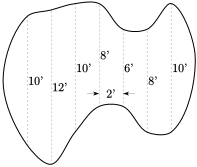
\includegraphics{pool}
\end{center}

\end{question}

\begin{hint}
See Section \eref{CLP101}{sec:Simpson} in the
%\href{http://www.math.ubc.ca/%7Efeldman/m101/clp/clp_notes_101.pdf}{CLP-2 text}.
CLP-2 text.
To set up the volume integral, see Example \eref{CLP101}{eg:VOLs} in the
%\href{http://www.math.ubc.ca/%7Efeldman/m101/clp/clp_notes_101.pdf}{CLP-2 text}.
CLP-2 text.

Since the cross-sections of the pool are semi-circular disks, a section that is $d$ metres across will have area $\frac{1}{2}\pi\left(\frac{d}{2}\right)^2$ square feet.  Based on the drawing, you may assume the very ends of the pool have distance 0 feet across.
\end{hint}

\begin{answer}
$\dfrac{472}{3}\approx 494 \ {\rm ft}^3$
\end{answer}

\begin{solution}
 Denote by $f(x)$ the width of the pool  $x$ feet
from the left-hand end. From the sketch, $f(0)=0$, $f(2)=10$, $f(4)=12$, $f(6)=10$,
$f(8)=8$, $f(10)=6$, $f(12)=8$, $f(14)=10$ and $f(16)=0$.

A cross-section of the pool $x$ feet from the left end is half of a circular disk with diameter $f(x)$ (so, radius $\frac{f(x)}{2}$) and thickness $\dee{x}$. So, the volume of
the part of the pool with $x$--coordinate running from $x$ to ($x+\dee{x}$) is
$\half\pi\big(\frac{f(x)}{2}\big)^2\,\dee{x} = \frac{\pi}{8}[f(x)]^2\,\dee{x}$.


The total volume is given by the following integral.
\begin{align*}
V&=\frac{\pi}{8}\int_0^{16}f(x)^2\,\dee{x}\cr
&\approx\frac{\pi}{8}\cdot\frac{\De x}{3}
\Big[f(0)^2+4f(2)^2+2f(4)^2+4f(6)^2+2f(8)^2
+4f(10)^2+2f(12)^2+4f(14)^2\!+f(16)^2\Big]\cr
&=\frac{\pi}{8}\cdot\frac{2}{3}
\Big[0+4(10)^2+2(12)^2+4(10)^2+2(8)^2
+4(6)^2+2(8)^2+4(10)^2+0\Big]\cr
&=\frac{472}{3}\pi\approx 494 \ {\rm ft}^3
\end{align*}

\end{solution}
%%%%%%%%%%%%%%%%%%%

\begin{Mquestion}[2002A,M121 2002A]
A piece of wire 1m long with radius 1mm is made in such
a way that the density varies in its cross-section, but is radially symmetric
(that is, the local density $g(r)$ in ${\rm kg/m^3}$ depends only on the
distance $r$ in mm from the centre of the wire). Take as given that the
total mass $W$ of the wire in kg is given by
\begin{align*}
W=2\pi 10^{-6}\int_0^1 rg(r)\,\dee{r}
\end{align*}
Data from the manufacturer is given below:

\renewcommand{\arraystretch}{1.1}
\begin{center}
     \begin{tabular}{|c|c|c|c|c|c|}
          \hline
          $r$ &0&1/4&1/2&3/4&1 \\
          \hline
          $g(r)$ &8051&8100&8144&8170&8190\\
          \hline
     \end{tabular}
\end{center}
\renewcommand{\arraystretch}{1.0}

\begin{enumerate}[(a)]
\item
Find the best Trapezoidal Rule approximation that you
can for $W$ based on the data in the table.
\item
Suppose that it is known that $|g'(r)|<200$ and
$|g''(r)|<150$ for all values of $r$. Determine the maximum possible size
of the error in the approximation you gave in part (a). Recall that if
a function $f(x)$ satisfies $|f''(x)|\le M$ on $[a,b]$, then
\begin{align*}
|I-T_n|\le\frac{M(b-a)^3}{12n^2}
\end{align*}
where $I=\int_a^b f(x)\,\dee{x}$ and $T_n$ is the Trapezoidal Rule approximation
to $I$ using $n$ subintervals.
\end{enumerate}
\end{Mquestion}

\begin{hint}
See Example \eref{CLP101}{eg:MidpointErr2} in the
%\href{http://www.math.ubc.ca/%7Efeldman/m101/clp/clp_notes_101.pdf}{CLP-2 text}.
CLP-2 text.

Don't get caught up in the interpretation of the integral. It's nice to see how integrals can be used, but for this problem, you're still just approximating the integral given, and bounding the error.

When you find the second derivative to bound your error, pay attention to the difference between the integrand and $g(r)$.
\end{hint}

\begin{answer}
(a) $0.025635$
\qquad (b) $1.8\times 10^{-5}$
\end{answer}

\begin{solution}
(a)
 The Trapezoidal Rule with $n=4$, $a=0$, $b=1$, and $\De x = \frac{1}{4}$ gives:
\begin{align*}
W=2\pi 10^{-6}\int_0^1 rg(r)\,\dee{r}
&\approx 2\pi 10^{-6}\De x\left[\frac{1}{2}x_0g(x_0)+x_1g(x_1)+x_2g(x_2)+x_3g(x_3)+ \frac{1}{2}x_4g(x_4)\right]\\
&=2\pi 10^{-6}\ \frac{1}{4}
\Big[\frac{1}{2} 0g(0)+\frac{1}{4}g\Big(\frac{1}{4}\Big)
+\frac{1}{2}g\Big(\frac{1}{2}\Big)+\frac{3}{4}g\Big(\frac{3}{4}\Big)
+\frac{1}{2} g(1)\Big] \\
&=\pi 10^{-6}\ \frac{1}{2}
\Big[\frac{8100}{4}
+\frac{8144}{2}+\frac{3\cdot 8170}{4}
+\frac{8190}{2} \Big] \\
& = \frac{32639\pi}{4\cdot 10^6}\approx 0.025635
\end{align*}

\noindent (b)
Using the product rule, the integrand $f(r)=2\pi 10^{-6} rg(r)$ obeys
\begin{align*}
f''(r)=2\pi 10^{-6} \diff{}{r}\big[g(r)+ rg'(r)\big]
=2\pi 10^{-6} \big[2g'(r)+ rg''(r)\big]
\end{align*}
and hence, for $0\le r\le 1$,
\begin{align*}
\big|f''(r)\big|\le 2\pi 10^{-6} \big[2\times200 + 1\times 150\big]
=1.1\pi 10^{-3}
\end{align*}
So,
\begin{align*}
|\text{Error}|\le \frac{1.1\pi 10^{-3}(1-0)^3}{12(4)^2}
\le1.8\times 10^{-5}
\end{align*}
\end{solution}
%%%%%%%%%%%%%%%%%%%%%%%%%%%%%%%%%%%%%%%%
%%%%%%%%%%%%%%%%%%%


\begin{Mquestion}[1997A]
Simpson's rule can be used to approximate $\log 2$,
since $\displaystyle\log 2=\int_1^2\frac{1}{x}\,\dee{x}$.
\begin{enumerate}[(a)]
\item
Use Simpson's rule with 6 subintervals to approximate $\log 2$.
\item
How many subintervals are required in order to guarantee
that the absolute error is less than $0.00001$?

\noindent  Note that if $E_n$ is the error using $n$ subintervals, then
$|E_n|\le\dfrac{L(b-a)^5}{180n^4}$ where $L$ is the maximum absolute value
of the fourth derivative of the function being integrated and $a$ and $b$
are the end points of the interval.
\end{enumerate}
\end{Mquestion}

\begin{hint}
See Example \eref{CLP101}{eg:SimpsonErr} in the
%\href{http://www.math.ubc.ca/%7Efeldman/m101/clp/clp_notes_101.pdf}{CLP-2 text}.
CLP-2 text. You'll want to use a calculator for the approximation in (a), and for finding the appropriate number of intervals in (b). Remember that Simpson's rule requires an even number of intervals.
\end{hint}

\begin{answer} (a)
$\approx 0.6931698$
\qquad (b)
$n\ge 12$ with $n$ even

\end{answer}

\begin{solution} (a)
Let $f(x)=\frac{1}{x}$, $a=1$, $b=2$ and
$\De x=\frac{b-a}{6}=\frac{1}{6}$. Using Simpson's rule:
\begin{align*}
\int_1^2\frac{1}{x}\ \dee{x}
&\approx \frac{\De x}{3}\Big[
f(1)+4f\Big(\frac{7}{6}\Big)+2f\Big(\frac{8}{6}\Big)
+4f\Big(\frac{9}{6}\Big)+2f\Big(\frac{10}{6}\Big)
+4f\Big(\frac{11}{6}\Big)+f(2)\Big]\\
&= \frac{1}{18}\Big[
1+\frac{24}{7}+\frac{12}{8}+\frac{24}{9}+\frac{12}{10}+\frac{24}{11}
+\frac{1}{2}\Big]\approx 0.6931698
\end{align*}

\noindent (b)
The integrand is $f(x)=\frac{1}{x}$. The first four derivatives
of $f(x)$ are:
\[f'(x)=-\frac{1}{x^2}, \qquad f''(x)=\frac{2}{x^3}, \qquad
f^{(3)}(x)=-\frac{6}{x^4}, \qquad f^{(4)}(x)=\frac{24}{x^5}\] On the interval
$1\le x\le 2$, the fourth derivative is never bigger in magnitude than
$L=24$.
\begin{align*}
|E_n|&\le\frac{L(b-a)^5}{180n^4}
=\frac{24(2-1)^5}{180n^4}
=\frac{4}{30n^4}
\intertext{So, we want an even number $n$ such that}
\frac{4}{30n^4} &\leq 0.00001 = \frac{1}{10^5}\\
n^4 & \geq \frac{40000}{3}\\
n&\geq \sqrt[4]{\frac{40000}{3}}\approx 10.7
\end{align*}
So, any even number greater than or equal to 12 will do.
\end{solution}

%%%%%%%%%%%%%%%%%%%


\begin{question}[1997D]
Let $I={\displaystyle\int_0^2}\cos(x^2)\ \dee{x}$ and
let $S_n$ be the Simpson's rule approximation to $I$ using $n$ subintervals.
\begin{enumerate}[(a)]
\item
Estimate the maximum absolute error in using $S_8$ to approximate $I$.
\item
How large should $n$ be in order to ensure that $|I-S_n|\le 0.0001$?
\end{enumerate}
\noindent  Note: The graph of $f''''(x)$, where $f(x)=\cos(x^2)$,
is shown below. The absolute error in the Simpson's rule approximation
is bounded by $\dfrac{L(b-a)^5}{180n^4}$ when $|f''''(x)|\le L$ on the
interval $[a,b]$.

\begin{center}
       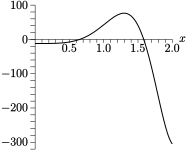
\includegraphics{graphE97D_11}
\end{center}

\end{question}

\begin{hint}
See Example \eref{CLP101}{eg:SimpsonErr} in the
%\href{http://www.math.ubc.ca/%7Efeldman/m101/clp/clp_notes_101.pdf}{CLP-2 text}.
CLP-2 text.

Rather than calculating the fourth derivative of the integrand, use the graph to find the largest absolute value it attains over our interval.
\end{hint}

\begin{answer} (a)
$0.01345$
\qquad (b)
 $n\ge 28$ with $n$ even

\end{answer}

\begin{solution} (a)
From the figure, we see that the magnitude of $|f''''(x)|$
never exceeds 310 for $0\le x\le 2$. So, the absolute error is bounded by
\begin{align*}
\frac{310(2-0)^5}{180\times 8^4}\le 0.01345
\end{align*}

\noindent (b)
We want to choose $n$ such that:
\begin{align*}
\frac{310(2-0)^5}{180\times n^4}&\le 10^{-4}\\
n^4&\ge \frac{310\times 2^5}{180}10^4\\
n&\ge 10\root 4 \of {\frac{310\times 32}{180}}\approx27.2
\end{align*}
For Simpson's rule, $n$ must be even, so any even integer obeying
$n\ge28$ will guarantee us the requisite accuracy.

\end{solution}
%%%%%%%%%%%%%%%%%%%

\begin{question}[2000D]
Define a function $f(x)$ and an integral $I$ by
\begin{align*}
f(x)=\int_0^{x^2}\sin(\sqrt{t})\,\dee{t},\qquad I=\int_0^1 f(t)\,\dee{t}
\end{align*}
Estimate how many subdivisions are needed to calculate $I$ to five decimal
places of accuracy using the trapezoidal rule.

\noindent  Note that if $E_n$ is the error using $n$ subintervals, then
$|E_n|\le\dfrac{M(b-a)^3}{12n^2\vphantom{\frac{1}{2}}}$, where $M$ is the maximum absolute value
of the second derivative of the function being integrated and $a$ and $b$
are the limits of integration.

\end{question}

\begin{hint}
See Example \eref{CLP101}{eg:MidpointErr2} in the
%\href{http://www.math.ubc.ca/%7Efeldman/m101/clp/clp_notes_101.pdf}{CLP-2 text}.
CLP-2 text.

You'll have to differentiate $f(x)$. To that end, you may also want to review the fundamental theorem of calculus
and, in particular, Example \eref{CLP101}{eg:INTftocB} in the
%\href{http://www.math.ubc.ca/%7Efeldman/m101/clp/clp_notes_101.pdf}{CLP-2 text}.
CLP-2 text.

You don't have to find the best possible value for $M$. A reasonable upper bound on $|f''(x)|$ will do.

To have five decimal places of accuracy, your error must be less than 0.000005. This ensures that, if you round your approximation to five decimal places, they will all be correct.
\end{hint}

\begin{answer}
$n\ge 259$
\end{answer}

\begin{solution}
Let $g(x)=\displaystyle\int_0^x\sin(\sqrt{t})\,\dee{t}$. By the Fundamental Theorem of Calculus Part 1,
$g'(x)= \sin(\sqrt{x})$. By its definition, $f(x)=g(x^2)$, so we use the chain rule to differentiate $f(x)$.
\begin{align*}
f'(x)=2xg'(x^2)=2x\sin x\qquad\qquad
f''(x)=2\sin x+2x\cos x
\end{align*}
Since $|\sin x|,|\cos x|\le 1$, we have
 $|f''(x)|\le 2+2|x|$ and, for $0\le t\le 1$, $|f''(t)|\le 4$. When the
trapezoidal rule with $n$ subintervals is applied, the resulting error $E_n$ obeys
\begin{align*}
E_n&\le\frac{4(1-0)^3}{12n^2}=\frac{1}{3n^2}
\intertext{We want an integer $n$ such that }
\frac{1}{3n^2}&\le 0.000005\\
n^2&\ge \frac{4}{12\times 0.000005}\\
n&\ge\sqrt{ \frac{1}{3\times 0.000005}} \approx258.2
\end{align*}
Any integer $n \geq 259$ will do.
\end{solution}
%%%%%%%%%%%%%%%%%%%%%%%%%%%%%%%%%%%%%%%%


\begin{question}\label{prob_s1.11_exactM}
%Let $f(x)=\frac{1}{6}x^3-\frac{1}{2}x^2-x+(1+x)\log|x+1|$.\\
Let $f(x)$ be a function\footnote{For example, $f(x)=\frac{1}{6}x^3-\frac{1}{2}x^2+(1+x)\log|x+1|$ will do, but you don't need to know what $f(x)$ is for this problem.} with $f''(x) = \dfrac{x^2}{x+1}$.

\begin{enumerate}[(a)]
\item Show that $|f''(x)| \leq 1$ whenever $x$ is in the interval $[0,1]$.
\item Find the maximum value of $|f''(x)|$ over the interval $[0,1]$.
\item Assuming $M=1$, how many intervals should you use to approximate $\displaystyle\int_{0}^{1}f(x)~\dee{x}$ to within $10^{-5}$?
\item Using the value of  $M$ you found in (b), how many intervals should you use to approximate $\displaystyle\int_0^1 f(x)~\dee{x}$ to within $10^{-5}$?\end{enumerate}

\end{question}
\begin{hint}
To find the maximum value of $|f''(x)|$, check its critical points and endpoints.
\end{hint}
\begin{answer}
(a) When $0 \leq x \leq1$, then $x^2 \leq 1$ and $x+1 \geq 1$, so $|f''(x)| = \dfrac{x^2}{|x+1|}\leq \dfrac{1}{1}=1$.\\
(b) $\dfrac{1}{2}$\qquad
(c) $n \geq 65$\qquad
(d) $n \geq 46$
\end{answer}
\begin{solution}


\begin{enumerate}[(a)]
\item When $0 \leq x \leq1$, then $x^2 \leq 1$ and $x+1 \geq 1$, so $|f''(x)| = \dfrac{x^2}{|x+1|}\leq \dfrac{1}{1}=1$.

\item
To find the maximum value of a function over a closed interval, we test the function's values at the endpoints of the interval and at its critical points inside the interval. The critical points are where the function's derivative is zero or does not exist.

The function we're trying to maximize is $|f''(x)| = \frac{x^2}{|x+1|} = \frac{x^2}{x+1}=f''(x)$ (since our interval only contains nonnegative numbers). So, the critical points occur when $f'''(x) = 0$ or does not exist. We find $f'''(x)$ Using the quotient rule.
\begin{align*}
f'''(x)&=\frac{(x+1)(2x)-x^2}{(x+1)^2}=\frac{x^2+2x}{(x+1)^2}\\
0&=\frac{x(x+2)}{x+1}\\
0&=x \quad\mbox{or}\quad x=-1\quad\mbox{or}\quad x=-2
\end{align*}
The only critical point in $[0,1]$ is $x=0$. So, the extrema of $f''(x)$ over $[0,1]$ will occur at its endpoints. Indeed, since $f'''(x) \geq 0$ for all $x$ in $[0,1]$, $f''(x)$ is increasing over this interval, so its maximum occurs at $x=1$. That is,
\[|f''(x)|\leq f''(1)=\frac{1}{2}\]

\item The absolute  error using the midpoint rule is at most $\dfrac{M(b-a)^3}{24n^2}$. Using $M=1$, if we want this to be no more than $10^{-5}$, we find an acceptable value of $n$ with the following calculation:
\begin{align*}
\dfrac{M(b-a)^3}{24n^2}&\leq 10^{-5}\\
\dfrac{1}{24n^2}&\leq 10^{-5}&(b-a=1,\,M=1)\\
\frac{10^5}{24} & \leq n^2\\
n & \geq 65
\end{align*}

\item The absolute  error using the midpoint rule is at most $\dfrac{M(b-a)^3}{24n^2}$. Using $M=\frac{1}{2}$, if we want this to be no more than $10^{-5}$, we find an acceptable value of $n$ with the following calculation:
\begin{align*}
\dfrac{M(b-a)^3}{24n^2}&\leq 10^{-5}\\
\dfrac{1}{48n^2}&\leq 10^{-5}&(b-a=1,\,M=\frac{1}{2})\\
\frac{10^5}{48} & \leq n^2\\
n & \geq 46
\end{align*}
\end{enumerate}
Remark: how accurate you want to be in these calculations depends a lot on your circumstances. Imagine, for instance, that you were finding $M$ by hand, using this to find $n$ by hand, then programming a computer to evaluate the approximation. For a simple integral like this, the difference between computing time for 65 intervals versus 46 is likely to be miniscule. So, there's not much to be gained by the extra work in (b). However, if your original sloppy $M$ gave you something like $n=1000000$, you might want to put some time into improving it, to shorten computation time. Moreover, if you were finding the approximation by hand, the difference between adding 46 terms and adding 65 terms would be considerable, and you would probably want to put in the effort up front to find the most accurate $M$ possible.
\end{solution}
%%%%%%%%%%%%%%%%%%%


\begin{Mquestion}
Approximate the function $\log x$ with a rational function by approximating the integral $\displaystyle\int_1^{x\vphantom{\frac{1}{2}}} \frac{1}{t}~\dee{t}$ using Simpson's rule. Your rational function $f(x)$  should approximate $\log x$ with an error of not more than 0.1 for any $x$ in the interval $[1,3]$.
\end{Mquestion}
\begin{hint}
In using Simpson's rule to approximate $\displaystyle\int_1^{x\vphantom{\frac{1}{2}}} \frac{1}{t}~\dee{t}$ with $n$ intervals, $a=1$, $b=x$, and $\De x = \dfrac{x-1}{n}$.
\end{hint}
\begin{answer}
$\displaystyle\frac{x-1}{12}\left[1+\frac{16}{x+3}+\frac{4}{x+1}+\frac{16}{3x+1}+\frac{1}{x}\right]$
\end{answer}
\begin{solution}
Before we can take our Simpson's rule approximation of $\displaystyle\int_1^x \dfrac{1}{t}~\dee{t}$, we need to know how many intervals to use. That means we need to bound our error, which means we need to bound $\ddiff{4}{}{t}\left\{\frac{1}{t}\right\}$.
\begin{align*}
\diff{}{t}\left\{\frac{1}{t}\right\}&=-\frac{1}{t^2}&
\ddiff{2}{}{t}\left\{\frac{1}{t}\right\}&=\frac{2}{t^3}\\
\ddiff{3}{}{t}\left\{\frac{1}{t}\right\}&=-\frac{6}{t^4}&
\ddiff{4}{}{t}\left\{\frac{1}{t}\right\}&=\frac{24}{t^5}
\end{align*}
So, over the interval $[1,3]$, $\displaystyle\left|\ddiff{4}{}{t}\left\{\frac{1}{t}\right\}\right| \leq 24$.

Now, we can find an appropriate $n$ to ensure our error will be be less than 0.1 for any $x$ in $[1,3]$:
\begin{align*}
\frac{L(b-a)^5}{180 n^4}&<0 .1
\\\frac{24(x-1)^5}{180 n^4}&< \frac{1}{10}
\\n^4 &> \frac{24\cdot (x-1)^5}{18}
\intertext{Because $x-1 \leq 2$ for every $x$ in $[1,3]$, if $n^4 > \dfrac{24\cdot 2^5}{18}$, then $n^4 > \dfrac{24\cdot (x-1)^5}{18}$ for every allowed $x$.}
n^4&>  \frac{24\cdot 2^5}{18}= \frac{128}{3}\\
n&>\sqrt[4]{\frac{128}{3}}\approx  2.6
\end{align*}
Since $n$ must be even, $n=4$ is enough intervals to guarantee our error is not too high for any $x$ in $[1,3]$. Now we find our Simpson's rule approximation with $n=4$, $a=1$, $b=x$,  and $\Delta x = \dfrac{x-1}{4}$. The points where we evaluate $\frac{1}{t}$ are:
\begin{align*}
x_0 =& 1 & x_1&=1+ \frac{x-1}{4}& x_2&=1+2\frac{x-1}{4}& x_3&=1+3\frac{x-1}{4}& x_4&=1+4\frac{x-1}{4}\\
&  & &=\frac{x+3}{4}& &=\frac{x+1}{2}&&=\frac{3x+1}{4}& &=x
\end{align*}

  \begin{center}
  \begin{tikzpicture}[scale=1.8]
  \draw[<->, thick] (-.5,0)--(8.5,0);
	\YExcoord{0}{\atp{1}{x_{0}}}
	\YExcoord{2}{\atp{\frac{x+3}{4}}{x_{1}}}
	\YExcoord{4}{\atp{\frac{x+1}{2}}{x_{2}}}
	\YExcoord{6}{\atp{\frac{3x+1}{4}}{x_{3}}}
	\YExcoord{8}{\atp{x}{x_{3}}}
  \end{tikzpicture}
  \end{center}

\begin{align*}
\log x=\int_1^x \frac{1}{t}~\dee{t}&\approx \frac{\De x}{3}\left[\frac{1}{x_0}+\frac{4}{x_1}+\frac{2}{x_2}+\frac{4}{x_3}+\frac{1}{x_4}\right]\\
&=\frac{x-1}{12}\left[1+\frac{16}{x+3}+\frac{4}{x+1}+\frac{16}{3x+1}+\frac{1}{x}\right]\\
&=f(x)
\end{align*}

Below is a graph of our approximation $f(x)$ and natural logarithm on the same axes. The natural logarithm function is shown red and dashed, while our approximating function is solid blue. Our approximation appears to be quite accurate for small, positive values of $x$.
\begin{center}
\begin{tikzpicture}
\YEaaxis{1}{11}{2}{6.5}
\draw[ultra thick, blue] plot[domain=.4:10.5, samples=100](\x,{2*(\x-1)/12*(1+16/(\x+3)+4/(\x+1)+16/(3*\x+1)+1/\x)}) node[above]{$y=f(x)$};
\draw[ultra thick, dashed, red] plot[domain=.4:10.5, samples=100](\x,{2*(ln \x)}) node[below]{$y=\log x$};
\foreach \x in {2,4,6,8,10}
	{\YExcoord{\x}{\x}}
\foreach \x in {1,2,3}
	{\YEycoord{2*\x}{\x}}
\end{tikzpicture}
\end{center}
\end{solution}
%%%%%%%%%%%%%%%%%%%


\begin{question}
Using an approximation of the area under the curve $\dfrac{1}{x^2+1}$, show that the constant $\arctan2$ is in the interval $\left[\dfrac{\pi}{4}+0.321,\, \dfrac{\pi}{4}+0.323\right]$.

You may assume use without proof that $\displaystyle\ddiff{4}{}{x}\left\{\frac{1}{1+x^2}\right\} = \dfrac{24(5x^4-10x^2+1)}{(x^2+1)^5}$. You may use a calculator, but only to add, subtract, multiply, and divide.
\end{question}
\begin{hint}
\begin{itemize}
\item $\int_1^2 \frac{1}{1+x^2}~\dee{x} = \arctan(2) - \frac{\pi}{4}$, so
$\arctan(2) = \frac{\pi}{4}+\int_1^2 \frac{1}{1+x^2}~\dee{x}$
\item If an approximation $A$ of the integral $ \int_1^2 \frac{1}{1+x^2}~\dee{x}$ has error at most $\varepsilon$, then $A-\varepsilon \leq \int_1^2 \frac{1}{1+x^2}~\dee{x} \leq A+\varepsilon$.
\item Looking at our target interval will tell you how small $\varepsilon$ needs to be, which in turn will tell you how many intervals you need to use.
\item You can show, by considering the numerator and denominator separately, that $|f^{(4)}(x)| \leq 30.75$ for every $x$ in $[1,2]$.
\item If you use Simpson's rule to approximate $\int_1^2 \frac{1}{1+x^2}~\dee{x}$, you won't need very many intervals to get the requisite accuracy.
\end{itemize}
\end{hint}
\begin{answer}
\Instructions{Note: for more detail, see the solutions.}

First, we use Simpson's rule with $n=4$  to approximate $\int_1^2 \frac{1}{1+x^2}\,\dee{x}$. The choice of this method (what we're approximating, why $n=4$, etc.) is explained in the solutions--here, we only show that it works.
\[\int_1^2 \frac{1}{1+x^2}\,\dee{x} \approx\frac{1}{12}\left[
\frac{1}{2} + \frac{64}{41}+\frac{8}{13}+\frac{64}{65}+\frac{1}{5}
\right]\approx 0.321748 \]
For ease of notation, define $A=0.321748$.

Now, we bound the error associated with this approximation. Define $N(x) = 24(5x^4-10x^2+1)$ and $D(x) = (x^2+1)^5$, so $N(x)/D(x)$ gives the fourth derivative of $\frac{1}{1+x^2}$. When $1 \le x \le 2$, $|N(x)| \le N(2)=984$ (because $N(x)$ is increasing over that interval) and $|D(x)| \geq D(1) = 2^5$ (because $D(x)$ is also increasing over that interval), so $\left| \ddiff{4}{}{x}\left\{\frac{1}{1+x^2}\right\}\right| = \left| \frac{N(x)}{D(x)}\right| \leq \frac{984}{2^5}=30.75$. Now we find the error bound for Simpson's rule with $L=30.75$, $b=2$, $a=1$, and $n=4$.
\[\left| \int_1^2 \frac{1}{1+x^2}\,\dee{x} - A\right| =|\text{error}| \leq \frac{L(b-a)^5}{180\cdot n^4}\
=\frac{30.75}{180\cdot 4^4}<0.00067\]
So,
\begin{align*}
-0.00067 &&<&&  \int_1^2 \frac{1}{1+x^2}\,\dee{x} - A &&<&& 0.00067\\
A-0.0067 &&<&&  \int_1^2 \frac{1}{1+x^2}\,\dee{x}  &&<&& A+0.00067\\
A-0.00067 &&<&& \arctan(2)-\arctan(1) &&<&& A+0.00067\\
A-0.00067 &&<&& \arctan(2)-\frac{\pi}{4} &&<&& A+0.00067\\
\frac{\pi}{4}+A-0.00067 &&<&& \arctan(2) &&<&&\frac{\pi}{4}+ A+0.00067\\
\frac{\pi}{4}+0.321748-0.00067 &&<&& \arctan(2) &&<&&\frac{\pi}{4}+0.321748+0.00067\\
\frac{\pi}{4}+0.321078 &&<&& \arctan(2) &&<&&\frac{\pi}{4}+0.322418\\
\frac{\pi}{4}+0.321 &&<&& \arctan(2) &&<&&\frac{\pi}{4}+0.323
\end{align*}
This was the desired bound.
\end{answer}
\begin{solution}
First, we want a strategy for approximating $\arctan 2$. Our hints are that involves integrating $\dfrac{1}{1+x^2}$, which is the antiderivative of arctangent, and the number $\dfrac{\pi}{4}$, which is the same as $\arctan(1)$. With that in mind:
\begin{align*}
\int_1^2 \frac{1}{1+x^2}~\dee{x}& = \arctan(2) - \arctan(1) = \arctan(2) - \frac{\pi}{4}\\
\text{So, }\qquad \arctan(2) &= \frac{\pi}{4} + \int_1^2 \frac{1}{1+x^2}~\dee{x}\tag{$*$}
\intertext{We won't know the value of the integral exactly, but we'll have an approximation $A$ bounded by some positive error bound $\varepsilon$. Then,}
 - \varepsilon &\leq \left(\int_1^2 \frac{1}{1+x^2}~\dee{x} - A\right) \leq \varepsilon\\
A - \varepsilon &\leq \left(\int_1^2 \frac{1}{1+x^2}~\dee{x}\right) \leq A + \varepsilon\\
 \text{So, from ($*$), }\qquad \frac{\pi}{4}+A-\varepsilon& \leq \arctan(2) \leq \frac{\pi}{4}+A+\varepsilon
\end{align*}

Which approximation should we use? We're given the fourth derivative of $\dfrac{1}{1+x^2}$, which is the derivative we need for Simpson's rule.  Simpson's rule  is also usually quite efficient, and we're very interested in not adding up dozens of terms, so we  choose Simpson's rule.

Now that we've chosen Simpson's rule, we should decide how many intervals to use.
In order to bound our error, we need to find a bound for the fourth derivative. To that end, define $N(x) = 24(5x^4-10x^2+1)$. Then $N'(x) = 24(20x^3-20x)= 480x(x^2-1)$, which is positive over the interval $[1,2]$. So, $N(x) \leq N(2)=24(5\cdot 2^4 - 10\cdot 2^2+1)=984$ when $1 \leq x \leq 2$. Furthermore, let $D(x)=(x^2+1)^5$. If  $1 \leq x \leq 2$, then $D(x) \geq 2^5$. Now we can find   a reasonable value of $L$:
\begin{align*}
|f^{(4)}(x)|&=\left|\frac{25(5x^4-10x^2+1)}{(x^2+1)^5}\right| =
\left|\frac{N(x)}{D(x)}\right| \leq \frac{984}{2^5} = \frac{123}{4} = 30.75
\end{align*}
So, we take $L=30.75$.



 We want $\left[\dfrac{\pi}{4}+A-\varepsilon ,\, \dfrac{\pi}{4}+A+\varepsilon \right]$ to look something like $\left[\dfrac{\pi}{4}+0.321,\, \dfrac{\pi}{4}+0.323\right]$. Note $\varepsilon$ is half the length of the first interval. Half the length of the second interval is $0.001 = \frac{1}{1000}$. So, we want a value of $\varepsilon$ that is no larger than this. Now we can find our $n$:
 \begin{align*}
\dfrac{L(b-a)^5}{180\cdot n^4} &\leq \frac{1}{1000}\\
\dfrac{30.75}{180\cdot n^4} &\leq \frac{1}{1000}\\
n^4 & \geq \frac{30.75\times 1000}{180}\\
n & \geq \sqrt[4]{\frac{30750}{180}}\approx 3.62
 \end{align*}

 So, we choose $n=4$), and are guaranteed that the absolute error in our approximation will be no more than $\dfrac{30.75}{180\cdot 4^4} < 0.00067$.

Since $n=4$, then $\De x = \dfrac{b-a}{n}=\dfrac{1}{4}$, so:
\[x_0 = 1 \qquad x_1=\frac{5}{4} \qquad x_2 = \frac{3}{2} \qquad x_3 = \frac{7}{4} \qquad x_4=2\]

Now we can find our Simpson's rule approximation $A$:
\begin{align*}
\int_0^1 \frac{1}{1+x^2}~\dee{x}&\approx \frac{\De x}{3}\big[
f(x_0) + 4f(x_1)+2f(x_2)+4f(x_3)+f(x_4)
\big]\\
&=\frac{1/4}{3}\big[
f(1) + 4f(5/4)+2f(3/2)+4f(7/4)+f(2)
\big]\\
&=\frac{1}{12}\left[
\frac{1}{1+1} + \frac{4}{25/16+1}+\frac{2}{9/4+1}+\frac{4}{49/16+1}+\frac{1}{4+1}
\right]\\
&=\frac{1}{12}\left[
\frac{1}{2} + \frac{4\cdot 16}{25+16}+\frac{2\cdot 4}{9+4}+\frac{4\cdot 16}{49+16}+\frac{1}{5}
\right]\\
&=\frac{1}{12}\left[
\frac{1}{2} + \frac{64}{41}+\frac{8}{13}+\frac{64}{65}+\frac{1}{5}
\right]\\
&\approx 0.321748=A
\end{align*}

As we saw before, the error associated with this approximation is at most $ \dfrac{30.75}{180\cdot 4^4} < 0.00067=\varepsilon$. So,
\begin{alignat*}{5}
&A-\varepsilon \quad&&\leq\quad && \int_1^2\frac{1}{1+x^2}~\dee{x}   &\leq \quad &A+\varepsilon&\\
\Rightarrow\qquad&0.321748 - 0.00067 \quad&&\leq\quad && \int_1^2\frac{1}{1+x^2}~\dee{x}  \quad &\leq \quad &0.321748 + 0.00067&\\
\Rightarrow\qquad&0.321078 &&\leq\quad & &\int_1^2\frac{1}{1+x^2}~\dee{x}\quad   &\leq \quad &0.322418&\\
\Rightarrow\qquad&0.321 &&\leq\quad  &&\int_1^2\frac{1}{1+x^2}~\dee{x}\quad   &\leq \quad &0.323&
\\\Rightarrow\qquad&\frac{\pi}{4}+0.321 && \leq\quad  &&\int_1^2\frac{1}{1+x^2}~\dee{x}+\frac{\pi}{4}\quad   &\leq \quad &\frac{\pi}{4}+0.323&
\\\\\Rightarrow\qquad&\frac{\pi}{4}+0.321 && \leq\quad &&\arctan(2)   &\leq \quad &\frac{\pi}{4}+0.323&
\end{alignat*}

This is precisely what we wanted to show.
\end{solution}
